% -*- coding: utf-8 -*-

\documentclass[10pt,dvipdfmx]{beamer}
\usepackage{tutorial}

\title{計算機実験I (第8回)}
\date{2020/06/17}

\begin{document}

\begin{frame}
  \titlepage
  \tableofcontents
\end{frame}

\begin{frame}[t]{本日の課題}
  \begin{itemize}
    %\setlength{\itemsep}{1em}
  \item 「\href{https://utphys-comp.github.io}{計算機実験のための環境整備}」({\small \href{https://utphys-comp.github.io}{https://utphys-comp.github.io}})が完了していない人は至急連絡を!
  \item 実習
    \begin{itemize}
    \item 実習課題一覧\href{https://github.com/todo-group/ComputerExperiments/releases/tag/2020s-computer1}{exercise-1.pdf}の課題17〜24 (あるいはそれ以外)から適宜選び実習
    \end{itemize}
  \item 質問はSlackの「\# 5\_対角化」あるいは他の適当と思われるチャンネルで \\[2em]
  \item レポートNo.3: 提出締切2020/7/3(金) 18:00 (レポート内容・提出方法についてはITC-LMSを参照のこと)
  \item 
  \end{itemize}
\end{frame}

\section{行列の対角化}
% -*- coding: utf-8 -*-

\documentclass[10pt,dvipdfmx]{beamer}
\usepackage{tutorial}

\begin{document}
\section{行列とLAPACK}
\begin{frame}[t,fragile]{二次元配列}
  \begin{itemize}
    %\setlength{\itemsep}{1em}
  \item C言語では、二次元配列は一次元配列の先頭をさす(ポインタ)の配列として表される(と理解しておけば良い)
  \item \verb+a[i]+は、要素\verb+a[i][0]+を指すポインタ
    \begin{itemize}
    \item \verb+a+ と \verb+&a[0]+ は等価 (\verb+&a[0][0]+ ではない)
    \item \verb+a[0]+ と \verb+&a[0][0]+ は等価
    \item \verb+a[2]+ と \verb+&a[2][0]+ は等価
    \item \verb^(a+2)^ と \verb^&a[2]^ は等価
    \item \verb^(*(a+2))[3]^ と \verb^*(*(a+2)+3)^ と \verb^a[2][3]^ は等価
    \item \verb^*(a+2)[3]^ と \verb^*((a+2)[3])^ と \verb^*(a[5])^ と\verb^a[5][0]^ は等価
    \item \verb^[]^は\verb^*^よりも優先度が高い
    \end{itemize}
  \item ポインタのテストプログラム: \href{https://github.com/todo-group/computer-experiments/blob/master/exercise/matrix/pointer-matrix.c}{pointer-matrix.c}
  \end{itemize}
\end{frame}

\begin{frame}[t,fragile]{動的二次元配列の確保}
  \begin{itemize}
    \setlength{\itemsep}{1em}
  \item 各行を表す配列とそれぞれの先頭アドレスを保持する配列の二種類が必要
\begin{lstlisting}
double **a;
m = 10;  
n = 10;  
a = (double**)malloc((size_t)(m * sizeof(double*));
for (int i = 0; i < m; ++i)
  a[i] = (double*)malloc((size_t)(n * sizeof(double));
\end{lstlisting}
\item 各行を保持する配列が、メモリ上で連続に確保される保証はない
\item 行列用のライブラリ(LAPACK等)を使うときに問題となる
  \end{itemize}
\end{frame}

\begin{frame}[t,fragile]{BLASライブラリ}
  \begin{itemize}
    \setlength{\itemsep}{1em}
  \item 行列・行列積、行列・ベクトル積などを高速に行う最適化された関数群
  \item 行列・行列積を計算するサブルーチン {\tt dgemm} \\
    \url{http://www.netlib.org/lapack/explore-html/d7/d2b/dgemm_8f.html}
    \begin{itemize}
    \item $C = \alpha A \times B + \beta C$ を計算
    \item BLASもFortranで書かれている
    \end{itemize}
  \item 例: \href{https://github.com/todo-group/computer-experiments/blob/master/exercise/matrix/multiply.c}{multiply.c}, \href{https://github.com/todo-group/computer-experiments/blob/master/exercise/matrix/multiply_dgemm.c}{multiply\_dgemm.c}
  \end{itemize}
\end{frame}

\begin{frame}[t,fragile]{LAPACK (Linear Algebra PACKage)}
  \begin{itemize}
    %\setlength{\itemsep}{1em}
  \item 線形計算のための高品質な数値計算ライブラリ
    \begin{itemize}
    \item \url{http://www.netlib.org/lapack}
    \item 線形方程式、固有値問題、特異値問題、線形最小二乗問題など
    \item (FFT 高速フーリエ変換は入っていない)
    % \item LAPACK自体もFortran言語で書かれている
    \end{itemize}
  \item ほぼ全てのPC、ワークステーション、スーパーコンピュータで利用可 (インストール済)
  \item Netlibでソースが公開されているリファレンス実装は遅いが、それぞれのベンダー(Intel、Fujitsu、etc)による最適化されたLAPACKが用意されている場合が多い(MKL、SSL2、etc)
  \item LAPACKを使うことにより、高速で信頼性が高く、ポータブルなコードを書くことが可能になる
  \end{itemize}
\end{frame}

\begin{frame}[t,fragile]{LAPACKによる連立一次方程式の求解}
  \begin{itemize}
    \setlength{\itemsep}{1em}
  \item LU分解を行うサブルーチン {\tt dgetrf} \\
    \url{http://www.netlib.org/lapack/explore-html/d3/d6a/dgetrf_8f.html}
  \item Fortranによる関数宣言
\begin{lstlisting}
subroutine dgetrf(integer M, integer N,
         double precision, dimension(lda, *) A,
         integer LDA, integer, dimension(*) IPIV,
         integer INFO)
\end{lstlisting}
\item {\tt A}: 左辺の行列、{\tt M,N}: 次元、{\tt IPIV}: 選択されたピボット行のリスト、{\tt lda}: 通常{\tt M} (行数)と同じで良い
  \end{itemize}
\end{frame}

\begin{frame}[t,fragile]{CからBLAS/LAPACKを呼び出す際の注意事項}
  \begin{itemize}
    %\setlength{\itemsep}{1em}
  \item (もともとFortran言語で書かれていたことによる制限)
  \item 関数名はすべて小文字、最後に \verb+_+ (下線)を付ける
  \item スカラー、ベクトル、行列は全て「ポインタ渡し」とする
  \item ベクトルや行列は最初の要素へのポインタを渡す (サイズは別に渡す)
  \item 行列の要素は(0,0) $\rightarrow$ (1,0) $\rightarrow$ (2,0) $\rightarrow\cdots\rightarrow$ $(m-1,0)$ $\rightarrow$ (0,1) $\rightarrow$ (1,1) $\rightarrow\cdots\rightarrow$ $(m-1,n-1)$の順で連続して並んでいなければならない(column-major)
    \begin{itemize}
    \item C言語の二次元配列では \verb+a[i][j]+ の次には \verb%a[i][j+1]%が入っている(row-major)
    \item 行列が転置されて解釈されてしまう!
    \end{itemize}
  \item コンパイル時には{\tt -llapack -lblas}オプションを指定し、LAPACKライブラリとBLASライブラリをリンクする(ハンドブック2.1.6節)
  \end{itemize}
\end{frame}

\begin{frame}[t,fragile]{cmatrix.hライブラリ}
  \begin{itemize}
    %\setlength{\itemsep}{1em}
  \item Column-major形式の二次元配列の確保({\tt alloc\_dmatrix})、開放({\tt free\_dmatrix})、出力({\tt print\_dmatrix})、読み込み({\tt read\_dmatrix})を行うためのユーティリティ関数、(i,j)成分にアクセスするためのマクロ({\tt mat\_elem})他を準備
  \item ソースコード: \href{https://github.com/todo-group/computer-experiments/blob/master/exercise/matrix/cmatrix.h}{cmatrix.h}
  \item 使用例
\begin{lstlisting}
#include "cmatrix.h"
...
double **mat;
mat = alloc_dmatrix(m, n);
mat_elem(mat, 1, 3) = 5.0;
...
free_dmatrix(mat);
\end{lstlisting}
  \item サンプルコード: \href{https://github.com/todo-group/computer-experiments/blob/master/exercise/matrix/matrix_example.c}{matrix\_example.c}
  \end{itemize}
\end{frame}

\begin{frame}[t,fragile]{alloc\_dmatrixでの動的二次元配列の確保}
  \begin{itemize}
    %\setlength{\itemsep}{1em}
  \item 長さ$m \times n$の一次元配列を用意し、各列(それぞれ$m$要素)の先頭アドレスを長さ$n$のポインター配列に格納する (ハンドブック2.12.3節)
\begin{lstlisting}
double **a;
m = 10;  
n = 10;  
a = (double**)malloc((size_t)(n * sizeof(double*));
a[0] = (double*)malloc((size_t)(m*n * sizeof(double));
for (int i = 1; i < n; ++i)
  a[i] = a[i-1] + m;
\end{lstlisting}
\item 行列の(i,j)成分を\verb+a[j][i]+に格納することにする (column-major)
  \end{itemize}
\end{frame}

\begin{frame}[t,fragile]{要素アクセス・先頭アドレス}
  \begin{itemize}
    % \setlength{\itemsep}{1em}
  \item 行列の(i,j)成分は\verb+a[j][i]+に格納されている
    \begin{itemize}
      \item \href{https://github.com/todo-group/computer-experiments/blob/master/exercise/matrix/cmatrix.h}{cmatrix.h}ではマクロ(\verb+mat_elem+)を準備
\begin{lstlisting}
#define mat_elem(mat, i, j) (mat)[j][i]
\end{lstlisting}
\item このマクロを使うと、例えば(i,j)成分への代入は以下のように書ける
\begin{lstlisting}
mat_elem(a, i, j) = 1;
\end{lstlisting}
\end{itemize}
  \item LAPACKにベクトルや行列の最初の要素へのポインタを渡す
    \begin{itemize}
      \item ベクトルの最初の要素(0)へのポインタ: \verb+&v[0]+
      \item 行列の最初の要素(0,0)へのポインタ: \verb+&a[0][0]+
      \item \href{https://github.com/todo-group/computer-experiments/blob/master/exercise/matrix/cmatrix.h}{cmatrix.h}にマクロ({\tt vec\_ptr}、{\tt mat\_ptr})が準備されているのでそれぞれ、{\tt vec\_ptr(v)}、{\tt mat\_ptr(a)}と書ける
    \end{itemize}
  \end{itemize}
\end{frame}

\begin{frame}[t,fragile]{LAPACKによる連立一次方程式の求解}
  \begin{itemize}
    \setlength{\itemsep}{1em}
  \item C言語から呼び出すための関数宣言を作成 (ハンドブック2.7.4節)
\begin{lstlisting}
void dgetrf_(int *M, int *N, double *A,
             int *LDA, int*IPIV, int *INFO);
\end{lstlisting}
関数名は全て小文字。関数名の最後に {\tt \_} (下線)を付ける
\item LU分解の例
\begin{lstlisting}
m = 10;
n = 10;
a = alloc_dmatrix(m, n);
...
dgetrf_(&m, &n, mat_ptr(a), &m, vec_ptr(ipiv), &info);
\end{lstlisting}
完全なソースコード: \href{https://github.com/todo-group/computer-experiments/blob/master/exercise/linear_system/lu_decomp.c}{lu\_decomp.c}
  \end{itemize}
\end{frame}

\end{document}


\section{特異値分解}

\begin{frame}[t,fragile]{一般の非正方行列の場合}
  \begin{itemize}
    %\setlength{\itemsep}{1em}
  \item 特異値分解(SVD: Singular Value Decomposition)
  \item 任意の$m \times n$実行列$A$は
    \[
    A = U \Lambda V^T
    \]
    の形に(一意に)分解できる ($k=\min(m,n)$)
  \item $U$: $(m \times k)$行列(列ベクトルは互いに正規直交) \\
    $V$: $(n \times k)$行列(列ベクトルは互いに正規直交) \\
    $\Lambda = \text{diag}(\lambda_1,\lambda_2,\cdots,\lambda_k)$ \ \ ($\lambda_1\ge\lambda_2\ge\cdots\ge\lambda_k\ge 0$) 特異値
  \item ベクトル表示 (行列をランク1の行列で分解)
    \[
    A = \sum_{i=1}^k \lambda_i u_i v_i^{T}
    \]
  \end{itemize}
\end{frame}

\begin{frame}[t,fragile]{特異値分解の例}
  \[
  \begin{split}
    \begin{pmatrix}
      1 & 2 & 3 \\
      6 & 4 & 5 \\
      8 & 9 & 7 \\
      10 & 11 & 12
    \end{pmatrix} =&
    \begin{pmatrix}
      -0.14 & -0.62 & -0.05 \\
      -0.34 & \ \ \,0.37 & \ \ \,0.81 \\
      -0.55 & \ \ \,0.54 & -0.58 \\
      -0.75 & -0.44 & \ \ \,0.06      
    \end{pmatrix} \\
    &\times
    \begin{pmatrix}
      25.35 & 0 & 0 \\
      0 & 2.15 & 0 \\
      0 & 0 & 1.71
    \end{pmatrix}
    \begin{pmatrix}
      -0.56 & -0.59 & -0.59 \\
      \ \ \,0.68 & \ \ \,0.09 & -0.73 \\
      \ \ \,0.48 & -0.81 & \ \ \,0.35
    \end{pmatrix}
  \end{split}
  \]
\end{frame}

\begin{frame}[t,fragile]{完全特異値分解 (full SVD)}
  \[
  \begin{split}
    \begin{pmatrix}
      1 & 2 & 3 \\
      6 & 4 & 5 \\
      8 & 9 & 7 \\
      10 & 11 & 12
    \end{pmatrix} =&
    \begin{pmatrix}
      -0.14 & -0.62 & -0.05 & {\color{red} -0.77} \\
      -0.34 & \ \ \,0.37 & \ \ \,0.81 & {\color{red} -0.29} \\
      -0.55 & \ \ \,0.54 & -0.58 & {\color{red} -0.29} \\
      -0.75 & -0.44 & \ \ \,0.06 & {\color{red} \ \ \,0.48}
    \end{pmatrix} \\
    &\times
    \begin{pmatrix}
      25.35 & 0 & 0 \\
      0 & 2.15 & 0 \\
      0 & 0 & 1.71 \\
      {\color{red} 0} & {\color{red} 0} & {\color{red} 0}
    \end{pmatrix}
    \begin{pmatrix}
      -0.56 & -0.59 & -0.59 \\
      \ \ \,0.68 & \ \ \,0.09 & -0.73 \\
      \ \ \,0.48 & -0.81 & \ \ \,0.35
    \end{pmatrix}
  \end{split}
  \]
  \begin{itemize}
    % \setlength{\itemsep}{1em}
  \item $U$, $V$が直交行列になるように、足りない基底ベクトルを追加
  \item こちらを「SVD」、もともとの分解を「thin SVD」と呼ぶこともある
  \end{itemize}
\end{frame}

\begin{frame}[t,fragile]{LAPACKによる特異値分解}
  \begin{itemize}
    %\setlength{\itemsep}{1em}
  \item 倍精度実行列の特異値分解 {\tt dgesvd}
    \url{http://www.netlib.org/lapack/explore-html/d8/d2d/dgesvd_8f.html}
  \item Fortranによる関数宣言
\begin{lstlisting}
subroutine dgesvd(character JOBU, character JOBVT,
  integer M, integer N,
  double precision, dimension(lda, *) A,
  integer LDA, double precision, dimension(*) S,
  double precision, dimension(ldu, *) U, integer LDU,
  double precision, dimension(ldvt, *) VT,
  integer LDVT,
  double precision, dimension(*) WORK, integer LWORK,
  integer INFO)
\end{lstlisting}
  \item {\tt dgesvd}の使用例: \href{https://github.com/todo-group/computer-experiments/blob/master/exercise/svd/svd.c}{svd.c} (SVD), \href{https://github.com/todo-group/computer-experiments/blob/master/exercise/svd/full_svd.c}{full\_svd.c} (完全SVD)
    \begin{itemize}
    \item コンパイル方法: {\tt cc -o svd svd.c -llapack -lblas -lm}
    \item 実行方法: {\tt ./svd matrix2.dat}
    \end{itemize}
  \end{itemize}
\end{frame}

\begin{frame}[t,fragile]{固有値分解との関係}
  \begin{itemize}
    %\setlength{\itemsep}{1em}
  \item 半正定値実対称行列の場合

    「固有値分解」と「特異値分解」は等価
  \item 一般の(非正方)実行列$A$の場合
    \begin{itemize}
      %\setlength{\itemsep}{1em}
    \item 完全SVD  $A=U \Lambda V^T$を考えると
    \item $B=A^T A = V \Lambda U^T U \Lambda V^T = V \Lambda^2 V^T$は実対称行列

      固有値:$\lambda_i^2$、固有ベクトル$V$
    \item $C=A A^T = U \Lambda V^T V \Lambda U^T = U \Lambda^2 U^T$も実対称行列

      固有値:$\lambda_i^2$、固有ベクトル$U$
    \end{itemize}
  \end{itemize}
\end{frame}

\begin{frame}[t,fragile]{特異値分解が役に立つ例}
  \begin{itemize}
    %\setlength{\itemsep}{1em}
  \item 連立一次方程式の最小二乗解
  \item 行列の低ランク近似
  \item 画像圧縮
  \end{itemize}
\end{frame}

\begin{frame}[t,fragile]{特異な(特異に近い)連立一次方程式}
  \begin{itemize}
    %\setlength{\itemsep}{1em}
  \item ランク$r$の$m \times n$行列$A$のfull SVDを考える
    \[
    A = \begin{pmatrix} U_1 U_2 \end{pmatrix} \begin{pmatrix} \Lambda_1 & 0 \\ 0 & 0 \end{pmatrix} \begin{pmatrix} V_1 V_2 \end{pmatrix}^T = U_1 \Lambda_1 V_1^T
    \]
    $U_1$: $m \times r$, $U_2$: $m \times (m-r)$, $\Lambda_1$: $r \times r$, $V_1$: $n \times r$, $V_2$: $n \times (n-r)$
  \item $r \ne n$のとき、方程式$Ax=b$は無限個の解をもつ、あるいは解なし
  \item 無限個の解をもつ場合($U_1U_1^Tb=b$)の一般解
    \[
    x = V_1 \Lambda_1^{-1} U_1^T b + V_2 z
    \]
    $z$は$(n-r)$次元の任意のベクトル
  \end{itemize}
\end{frame}

\begin{frame}[t,fragile]{一般化逆行列と最小二乗解}
  \begin{itemize}
    %\setlength{\itemsep}{1em}
  \item $V_1$と$V_2$の列ベクトルは全て直交する。一般解のうちノルム$|x|^2$が最小となるのは$z=0$のとき
    \[
    x = A^\dagger b \ \ \ \ A^\dagger = V \begin{pmatrix} \Lambda^{-1} & 0 \\ 0 & 0 \end{pmatrix} U^T
    \]
  \item $A^\dagger$: Moore-Penroseの一般化逆行列 (1/0を0とおくことに相当)
  \item $Ax=b$が解を持たない場合にも最良解を与える
  \item 零に非常に近い特異値がある場合も、それらを零とみなすことで数値的に安定した解がえられる
  \end{itemize}
\end{frame}

\begin{frame}[t,fragile]{行列の低ランク近似}
  \begin{itemize}
    %\setlength{\itemsep}{1em}
  \item ランク$r$ ($r<k$)の行列のうち、行列$A$を「最も良く近似」する$\tilde{A}$を選ぶ
  \item 「最も良く近似」= フロベニウスノルム$||A-\tilde{A}||_\mathrm{F}$を最小化
    \[
    ||X||^2_\mathrm{F} \equiv \sum_{ij} x_{ij}^2
    \]
  \item 特異値のうち大きなものから$r$個とり、残りを零とした
    \[
    \tilde{\Lambda} = \text{diag}(\lambda_1,\cdots,\lambda_r,0,\cdots,0)
    \]
    を使い
    \[
    \tilde{A} = U \tilde{\Lambda} V^T
    \]
    を作れば良い (Eckart-Youngの定理)
  \end{itemize}
\end{frame}

\begin{frame}[t,fragile]{行列の低ランク近似の例}
  \[
  \begin{split}
    &\begin{pmatrix}
      -0.14 & -0.62 & -0.05 \\
      -0.34 & \ \ \,0.37 & \ \ \,0.81 \\
      -0.55 & \ \ \,0.54 & -0.58 \\
      -0.75 & -0.44 & \ \ \,0.06      
    \end{pmatrix}
    \begin{pmatrix}
      25.35 & 0 & 0 \\
      0 & 2.15 & 0 \\
      0 & 0 & 0
    \end{pmatrix} \\
    & \times
    \begin{pmatrix}
      -0.56 & -0.59 & -0.59 \\
      \ \ \,0.68 & \ \ \,0.09 & -0.73 \\
      \ \ \,0.48 & -0.81 & \ \ \,0.35
    \end{pmatrix}
    = 
    \begin{pmatrix}
      1.04 & 1.93 & 3.03 \\
      5.33 & 5.12 & 4.52 \\
      8.47 & 8.21 & 7.34 \\
      9.95 & 11.1 & 12.0 \\
    \end{pmatrix}
  \end{split}
  \]
  \begin{itemize}
    % \setlength{\itemsep}{1em}
  \item それなりに悪くない近似が得られる
  \item 誤差(フロベニウスノルム) = 1.71 (無視した特異値の二乗和の平方根)
  \end{itemize}
\end{frame}

\begin{frame}[t,fragile]{Eckart-Youngの定理の証明}
  \begin{itemize}
    %\setlength{\itemsep}{1em}
  %\item $A=U \Lambda V^T$のように(完全)SVDされているとする
  \item $A$を近似する行列$X$ (ランク$\le r$)を考えると
    \[
    ||A-X||_\mathrm{F}^2 = \sum_{ij}(a_{ij}-x_{ij})^2 = \text{tr} [(A-X)(A-X)^T]
    \]
    を最小化すればよい。完全SVDについて$UU^T=E_m$, $VV^T = E_n$より
    \[
    \begin{split}
      ||A-X||_\mathrm{F}^2 &= \text{tr} [UU^T(A-X)VV^T(A-X)^T] \\
      %% &= \text{tr} [U^T(A-X)V (U^T(A-X)V)^T] \\
      &= \text{tr} [(\Lambda-G)(\Lambda-G)^T]  \ \ \ (G \equiv U^TXV)\\
      &= \sum_i^k (\lambda_i - g_{ii})^2 + \sum_i \sum_{j \ne i} g_{ij}^2
    \end{split}
    \]
    ランク$r$以下で、$||A-X||_\mathrm{F}^2$を最小化するには、$g_{ii}=\lambda_i$ ($i=1 \cdots r$)、それ以外は全て零とすればよい
  \end{itemize}
\end{frame}

\begin{frame}[t,fragile]{特異値分解による画像圧縮}
  \begin{itemize}
  \item 特異値の分布とランク$r$近似 ($1614 \times 2178$グレイスケール写真)
    
    \hspace*{-3em}\resizebox{0.27\textwidth}{!}{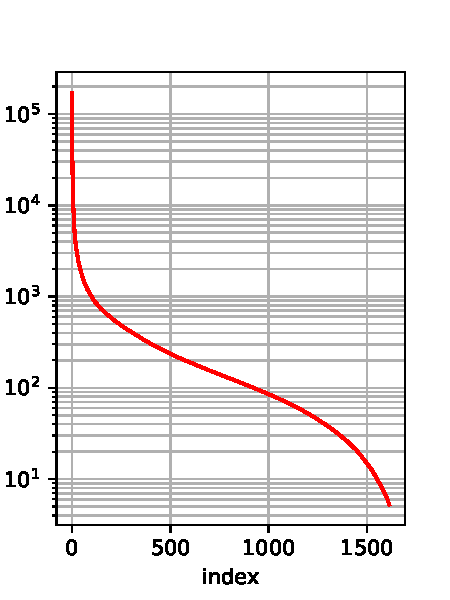
\includegraphics{image/singular_values.pdf}}

    \vspace*{-11em}\hfill
    \begin{tabular}{cccc}
      $r=1$ & $r=2$ & $r=3$ & $r=4$ \\
      \resizebox{0.15\textwidth}{!}{
\includegraphics{image/gray_picture_r1.pdf}} &
      \resizebox{0.15\textwidth}{!}{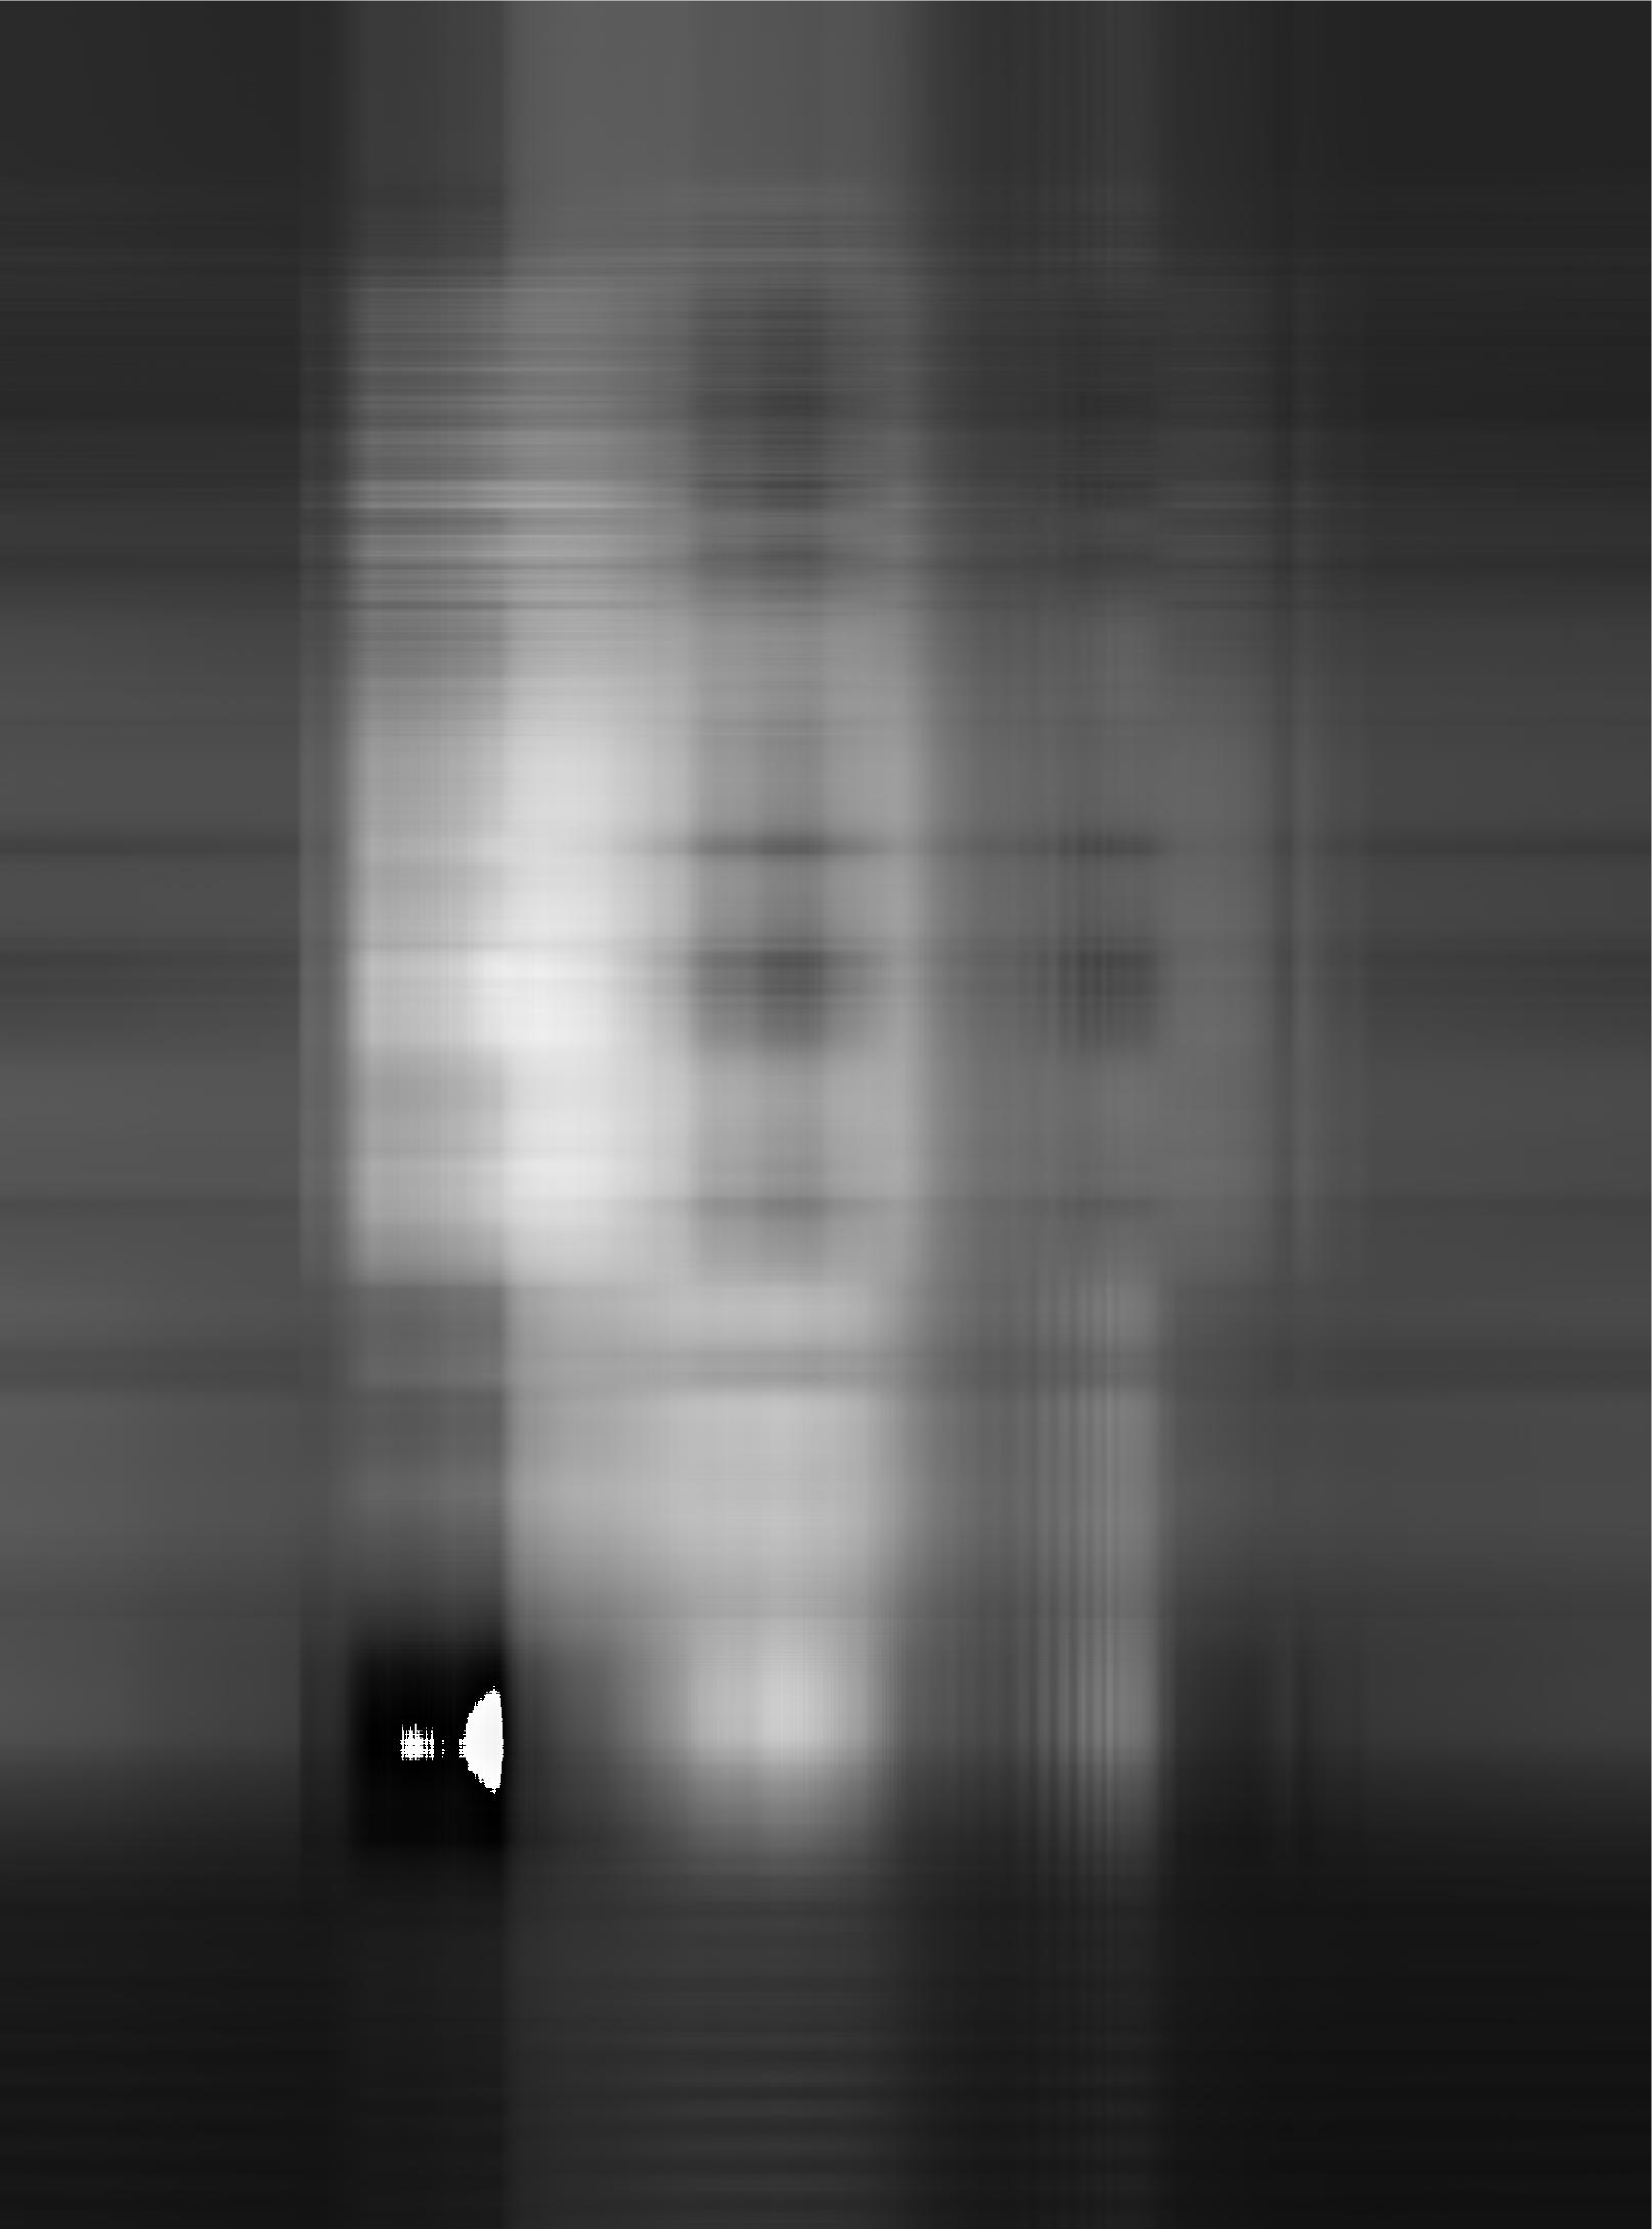
\includegraphics{image/gray_picture_r2.pdf}} &
      \resizebox{0.15\textwidth}{!}{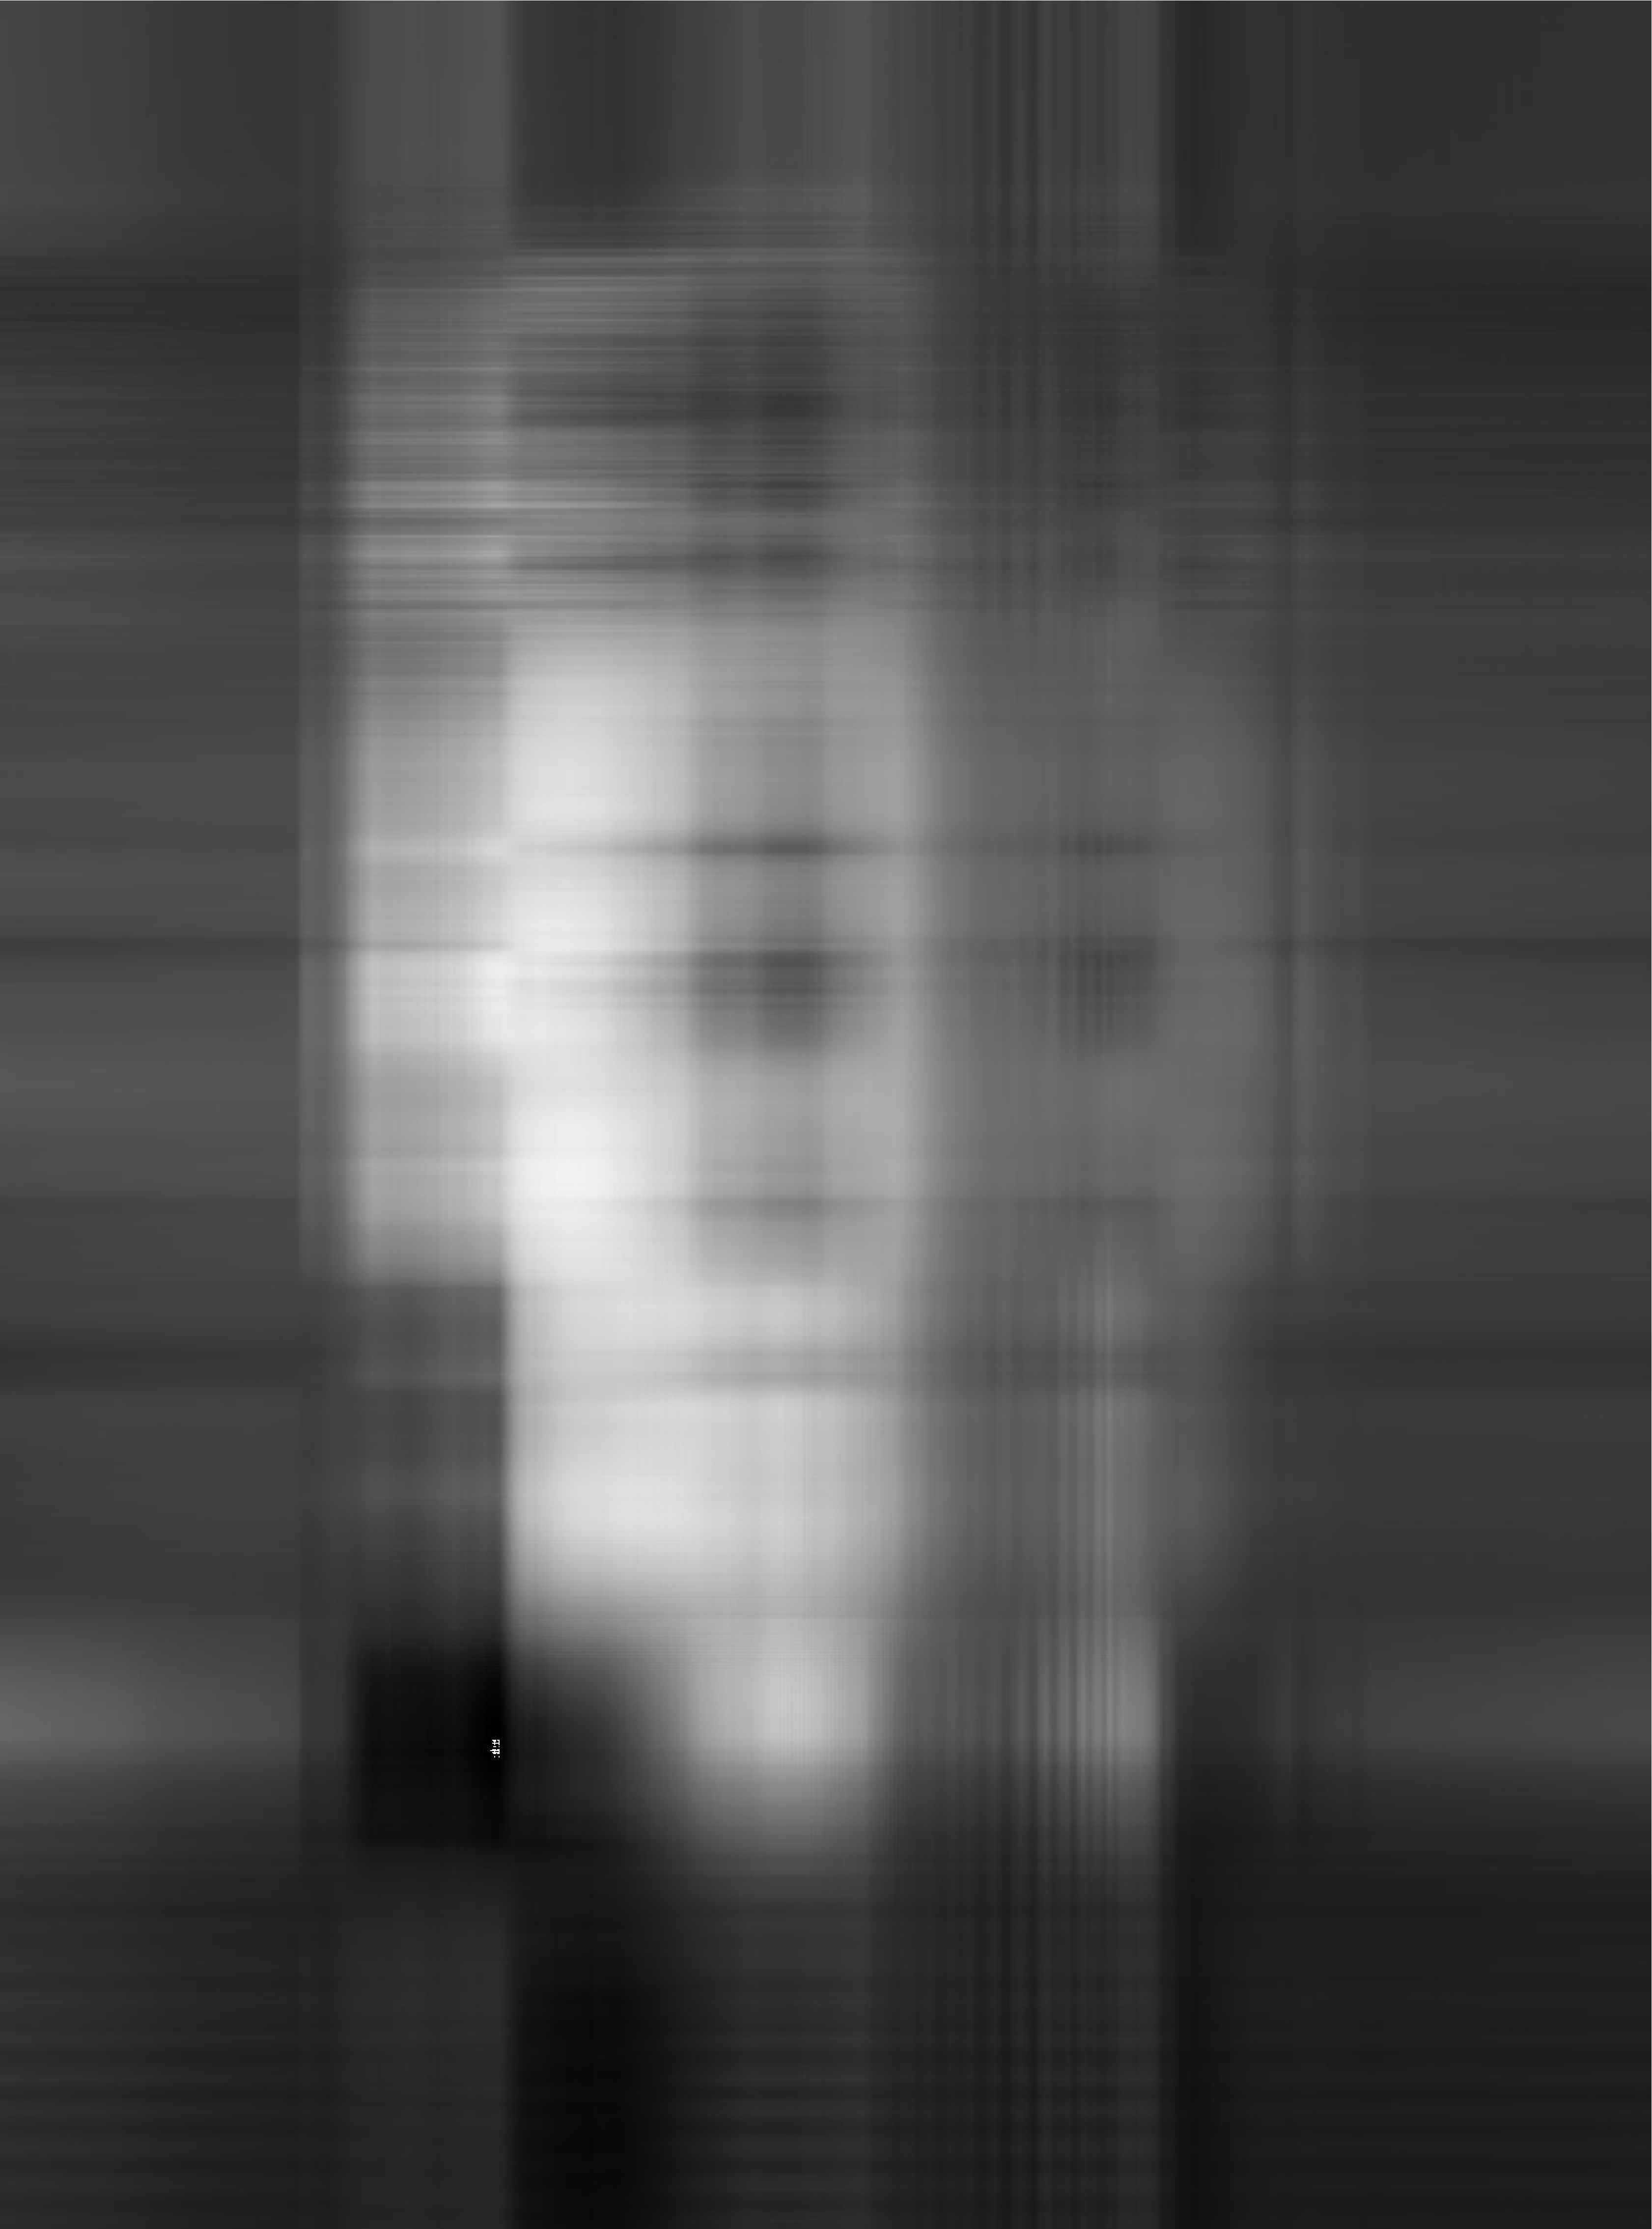
\includegraphics{image/gray_picture_r3.pdf}} &
      \resizebox{0.15\textwidth}{!}{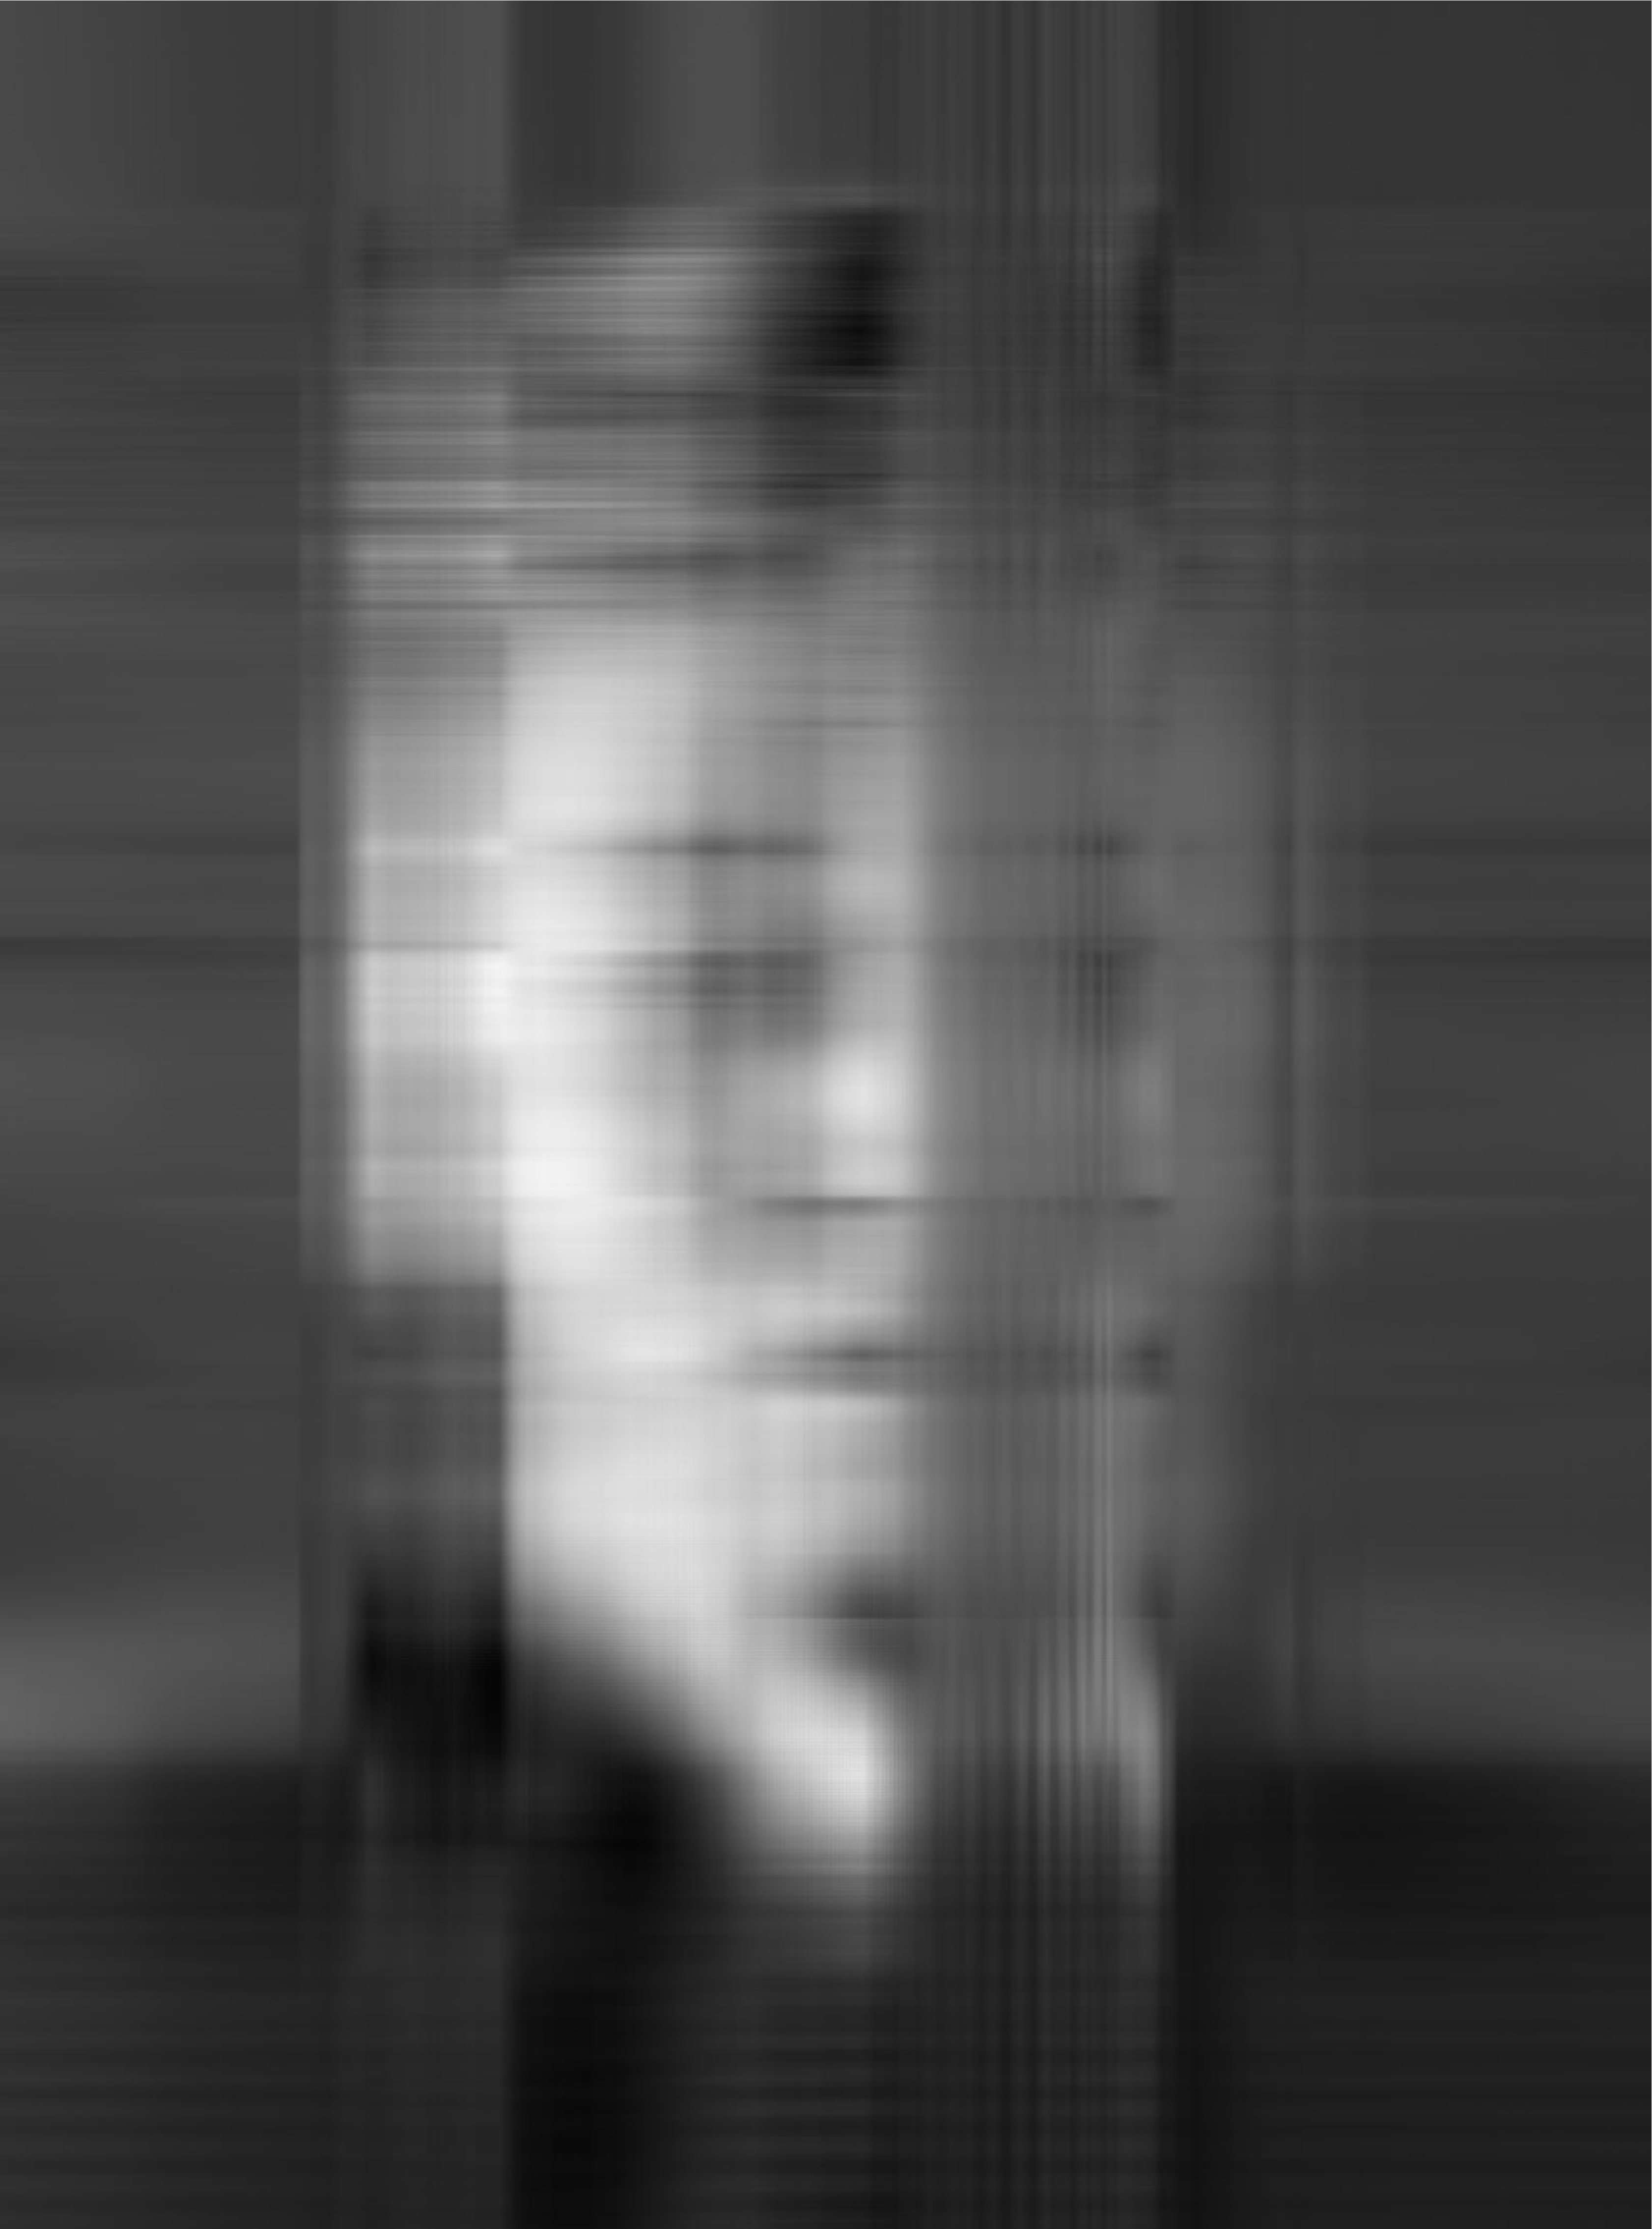
\includegraphics{image/gray_picture_r4.pdf}} \\
    \end{tabular}
  \end{itemize}
\end{frame}

\begin{frame}[t,fragile]{特異値分解による画像圧縮}
  \begin{itemize}
  \item 特異値の分布とランク$r$近似 ($1614 \times 2178$グレイスケール写真)
    
    \hspace*{-3em}\resizebox{0.27\textwidth}{!}{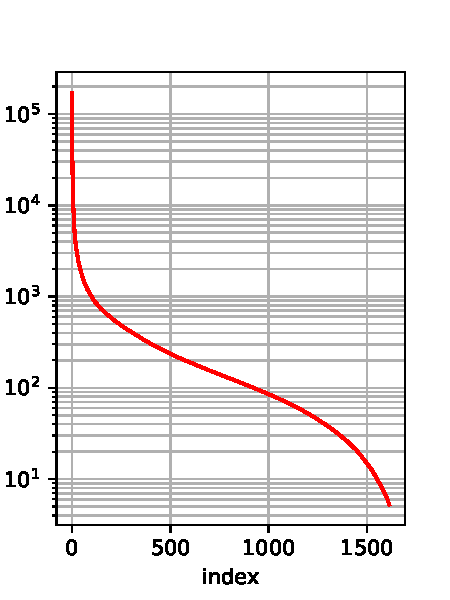
\includegraphics{image/singular_values.pdf}}

    \vspace*{-11em}\hfill
    \begin{tabular}{cccc}
      $r=1$ & $r=2$ & $r=3$ & $r=4$ \\
      \resizebox{0.15\textwidth}{!}{
\includegraphics{image/gray_picture_r1.pdf}} &
      \resizebox{0.15\textwidth}{!}{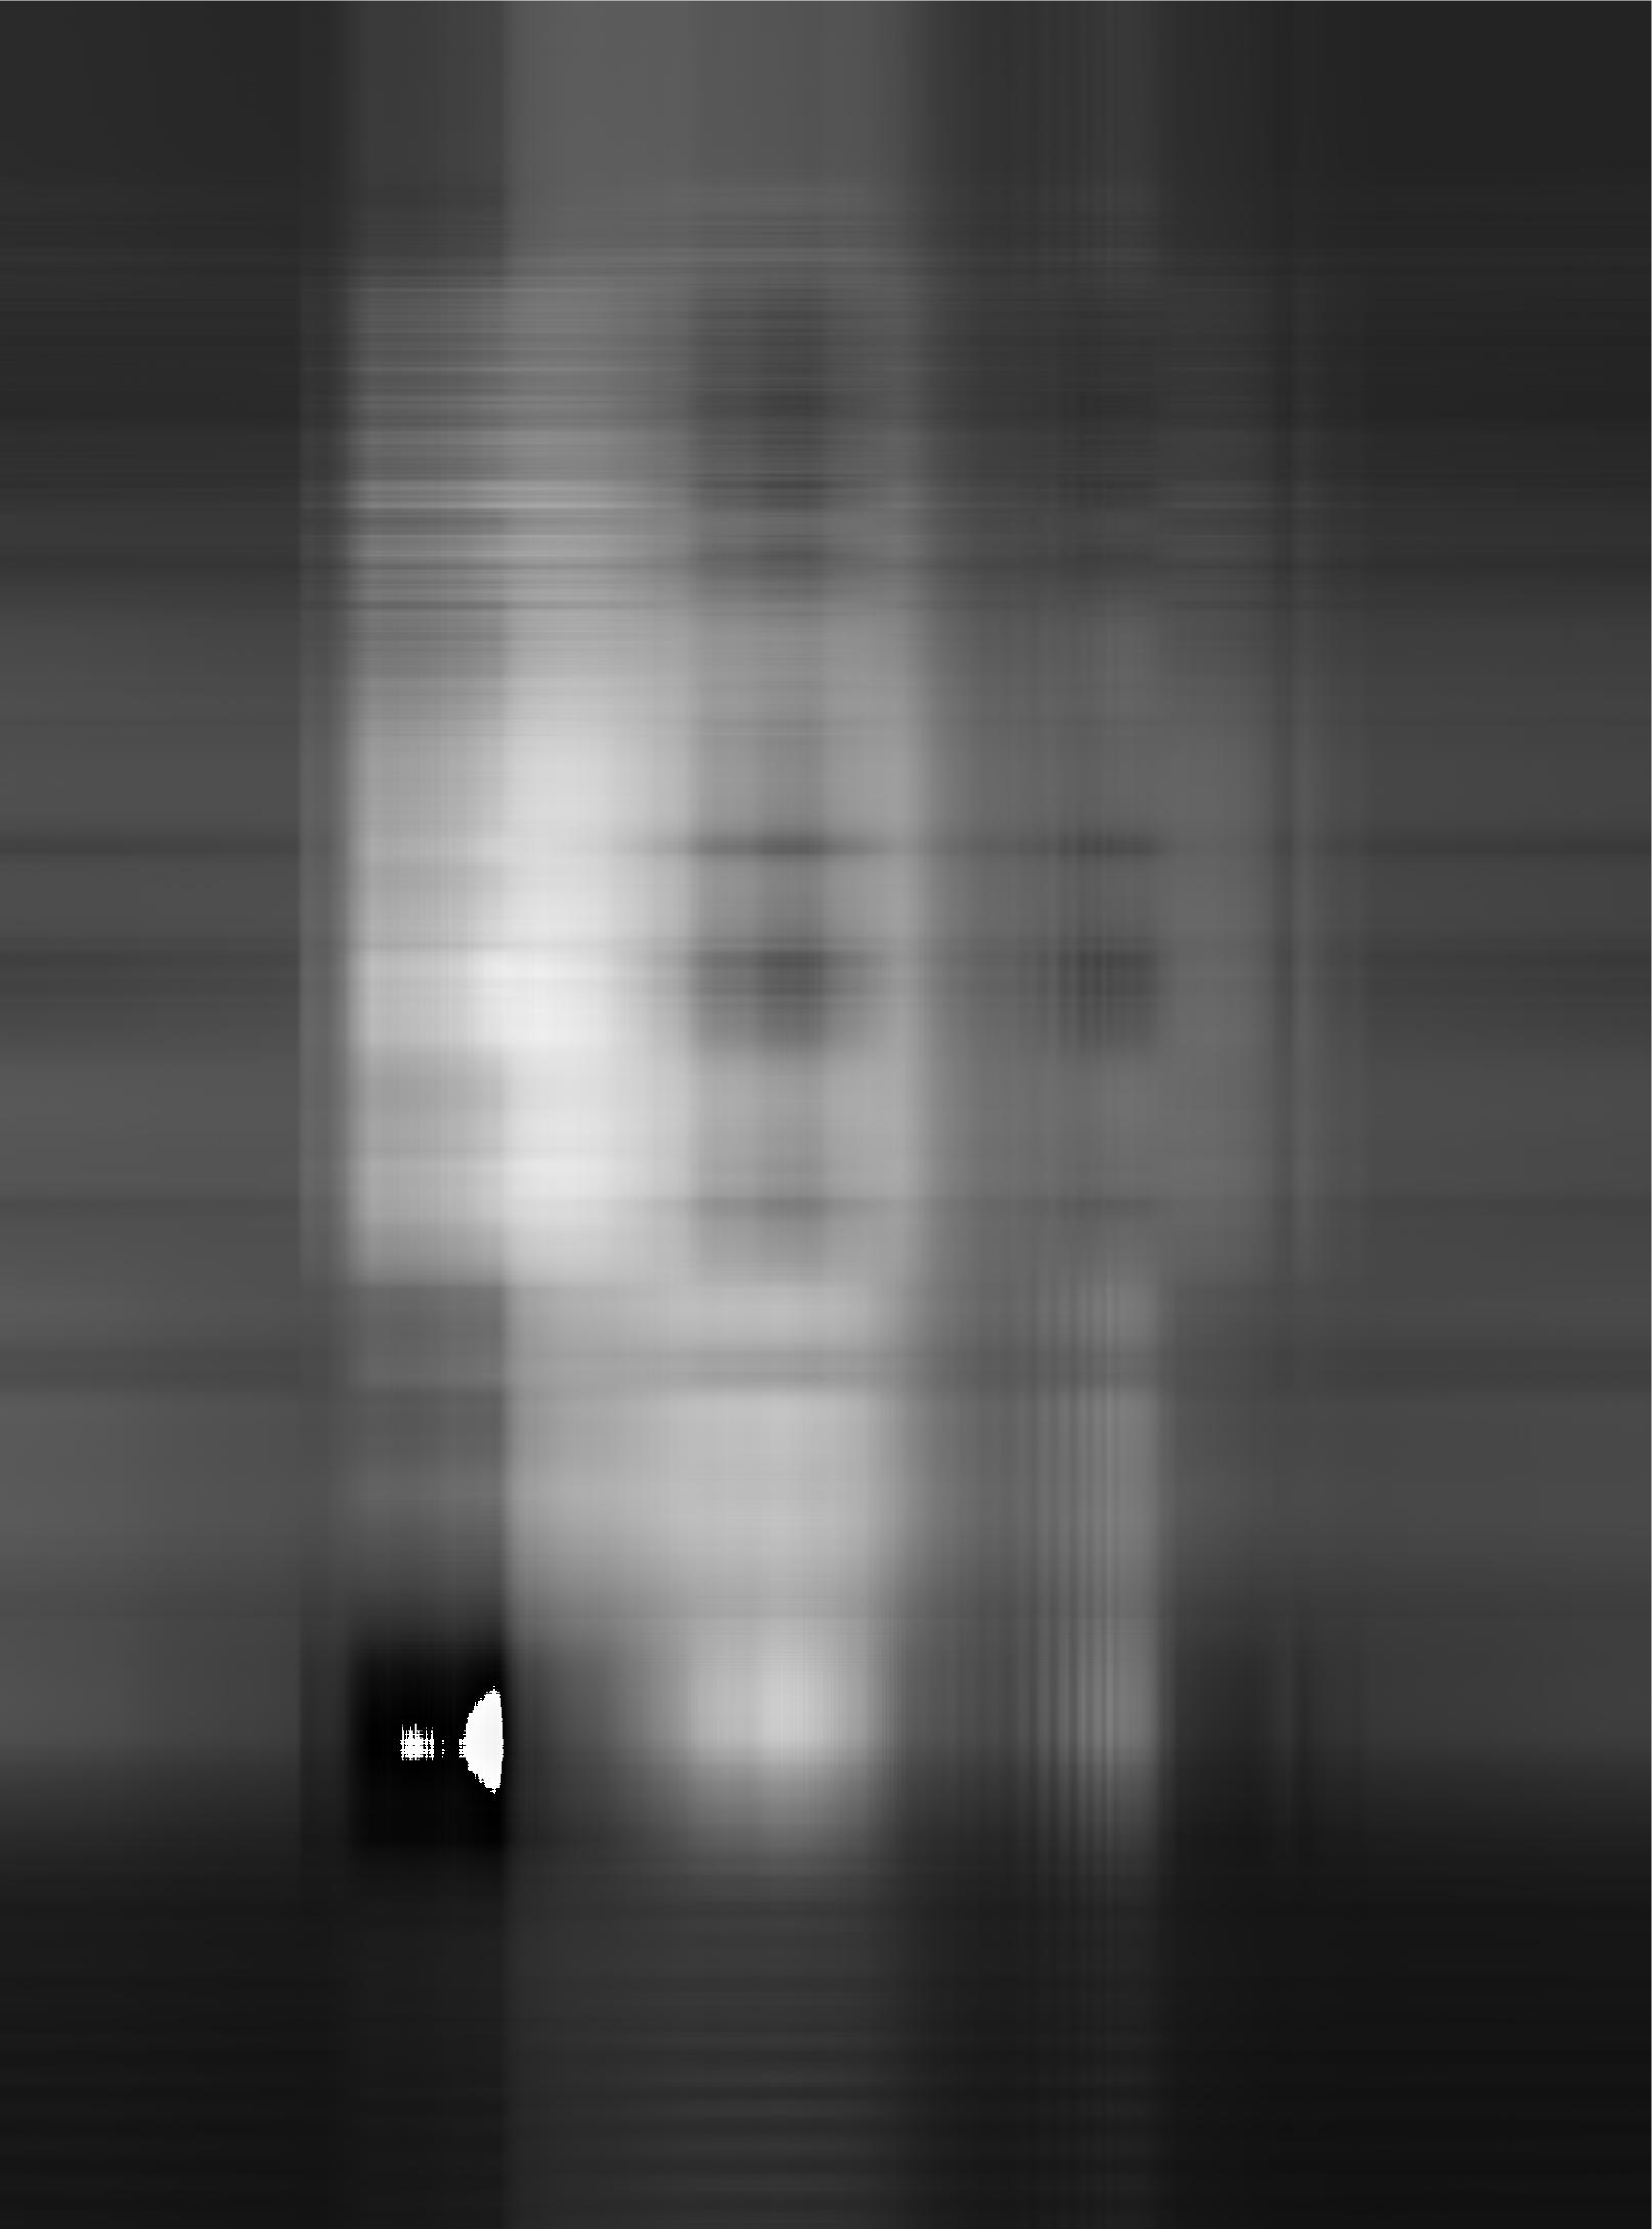
\includegraphics{image/gray_picture_r2.pdf}} &
      \resizebox{0.15\textwidth}{!}{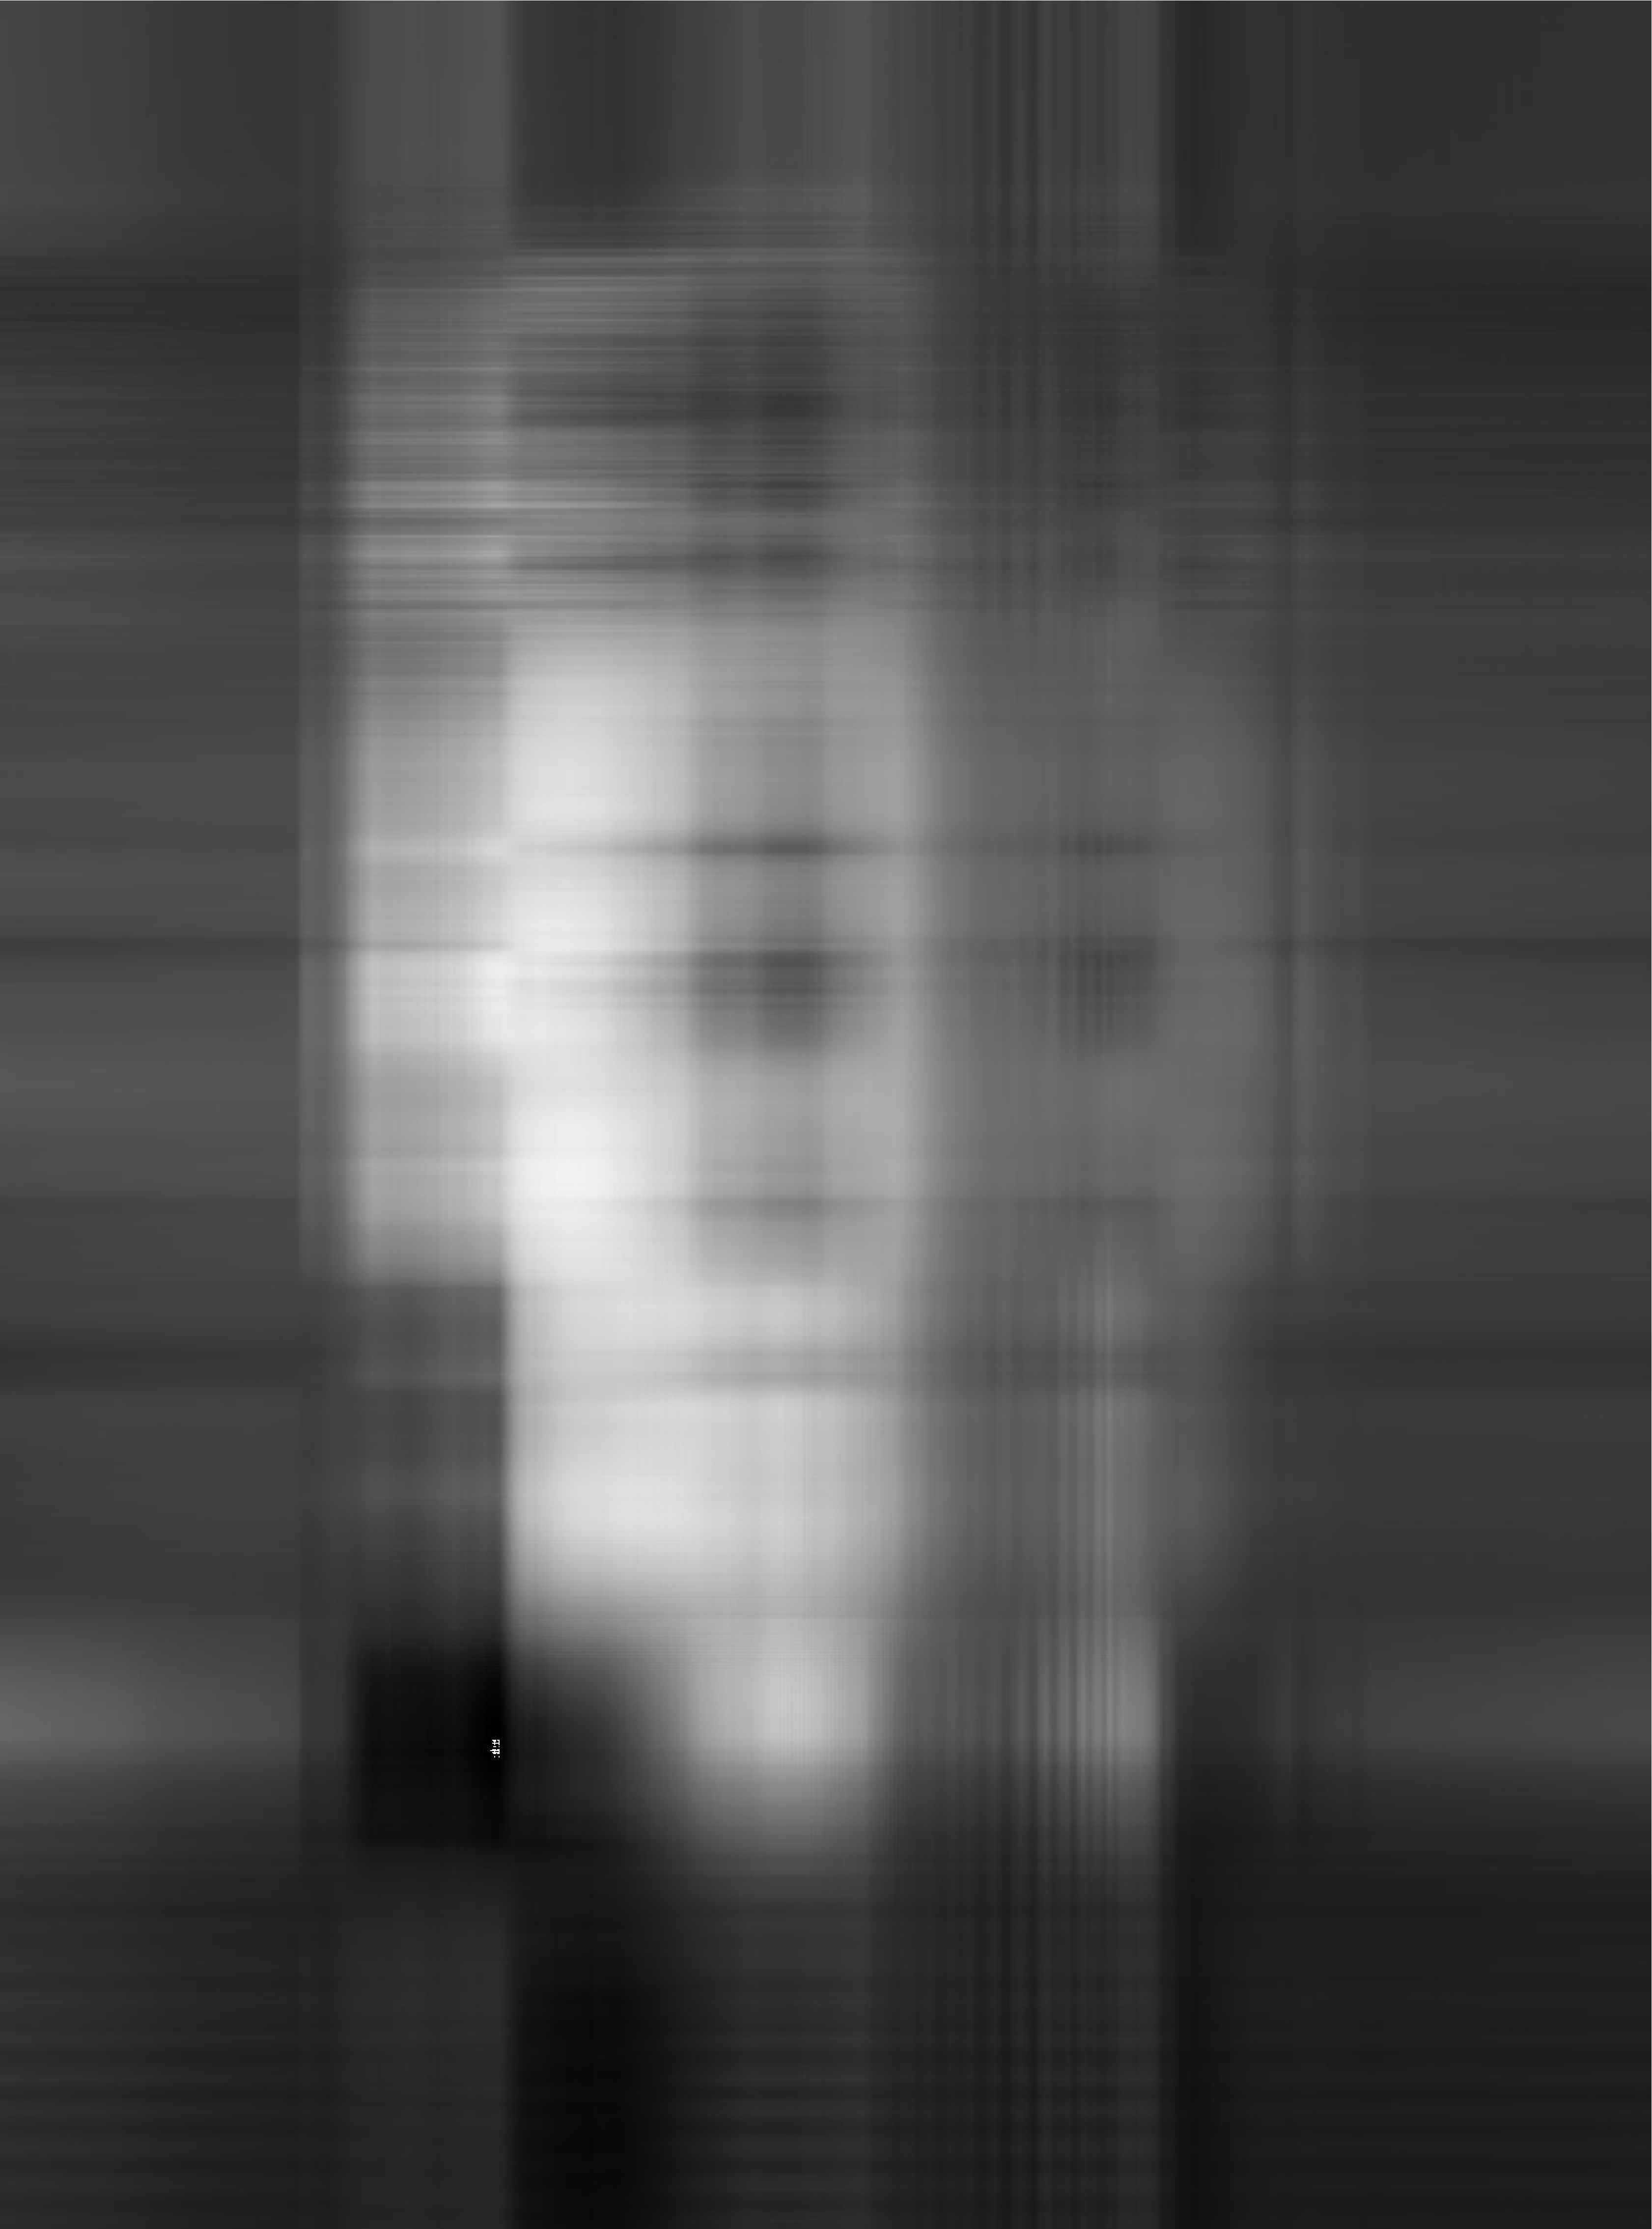
\includegraphics{image/gray_picture_r3.pdf}} &
      \resizebox{0.15\textwidth}{!}{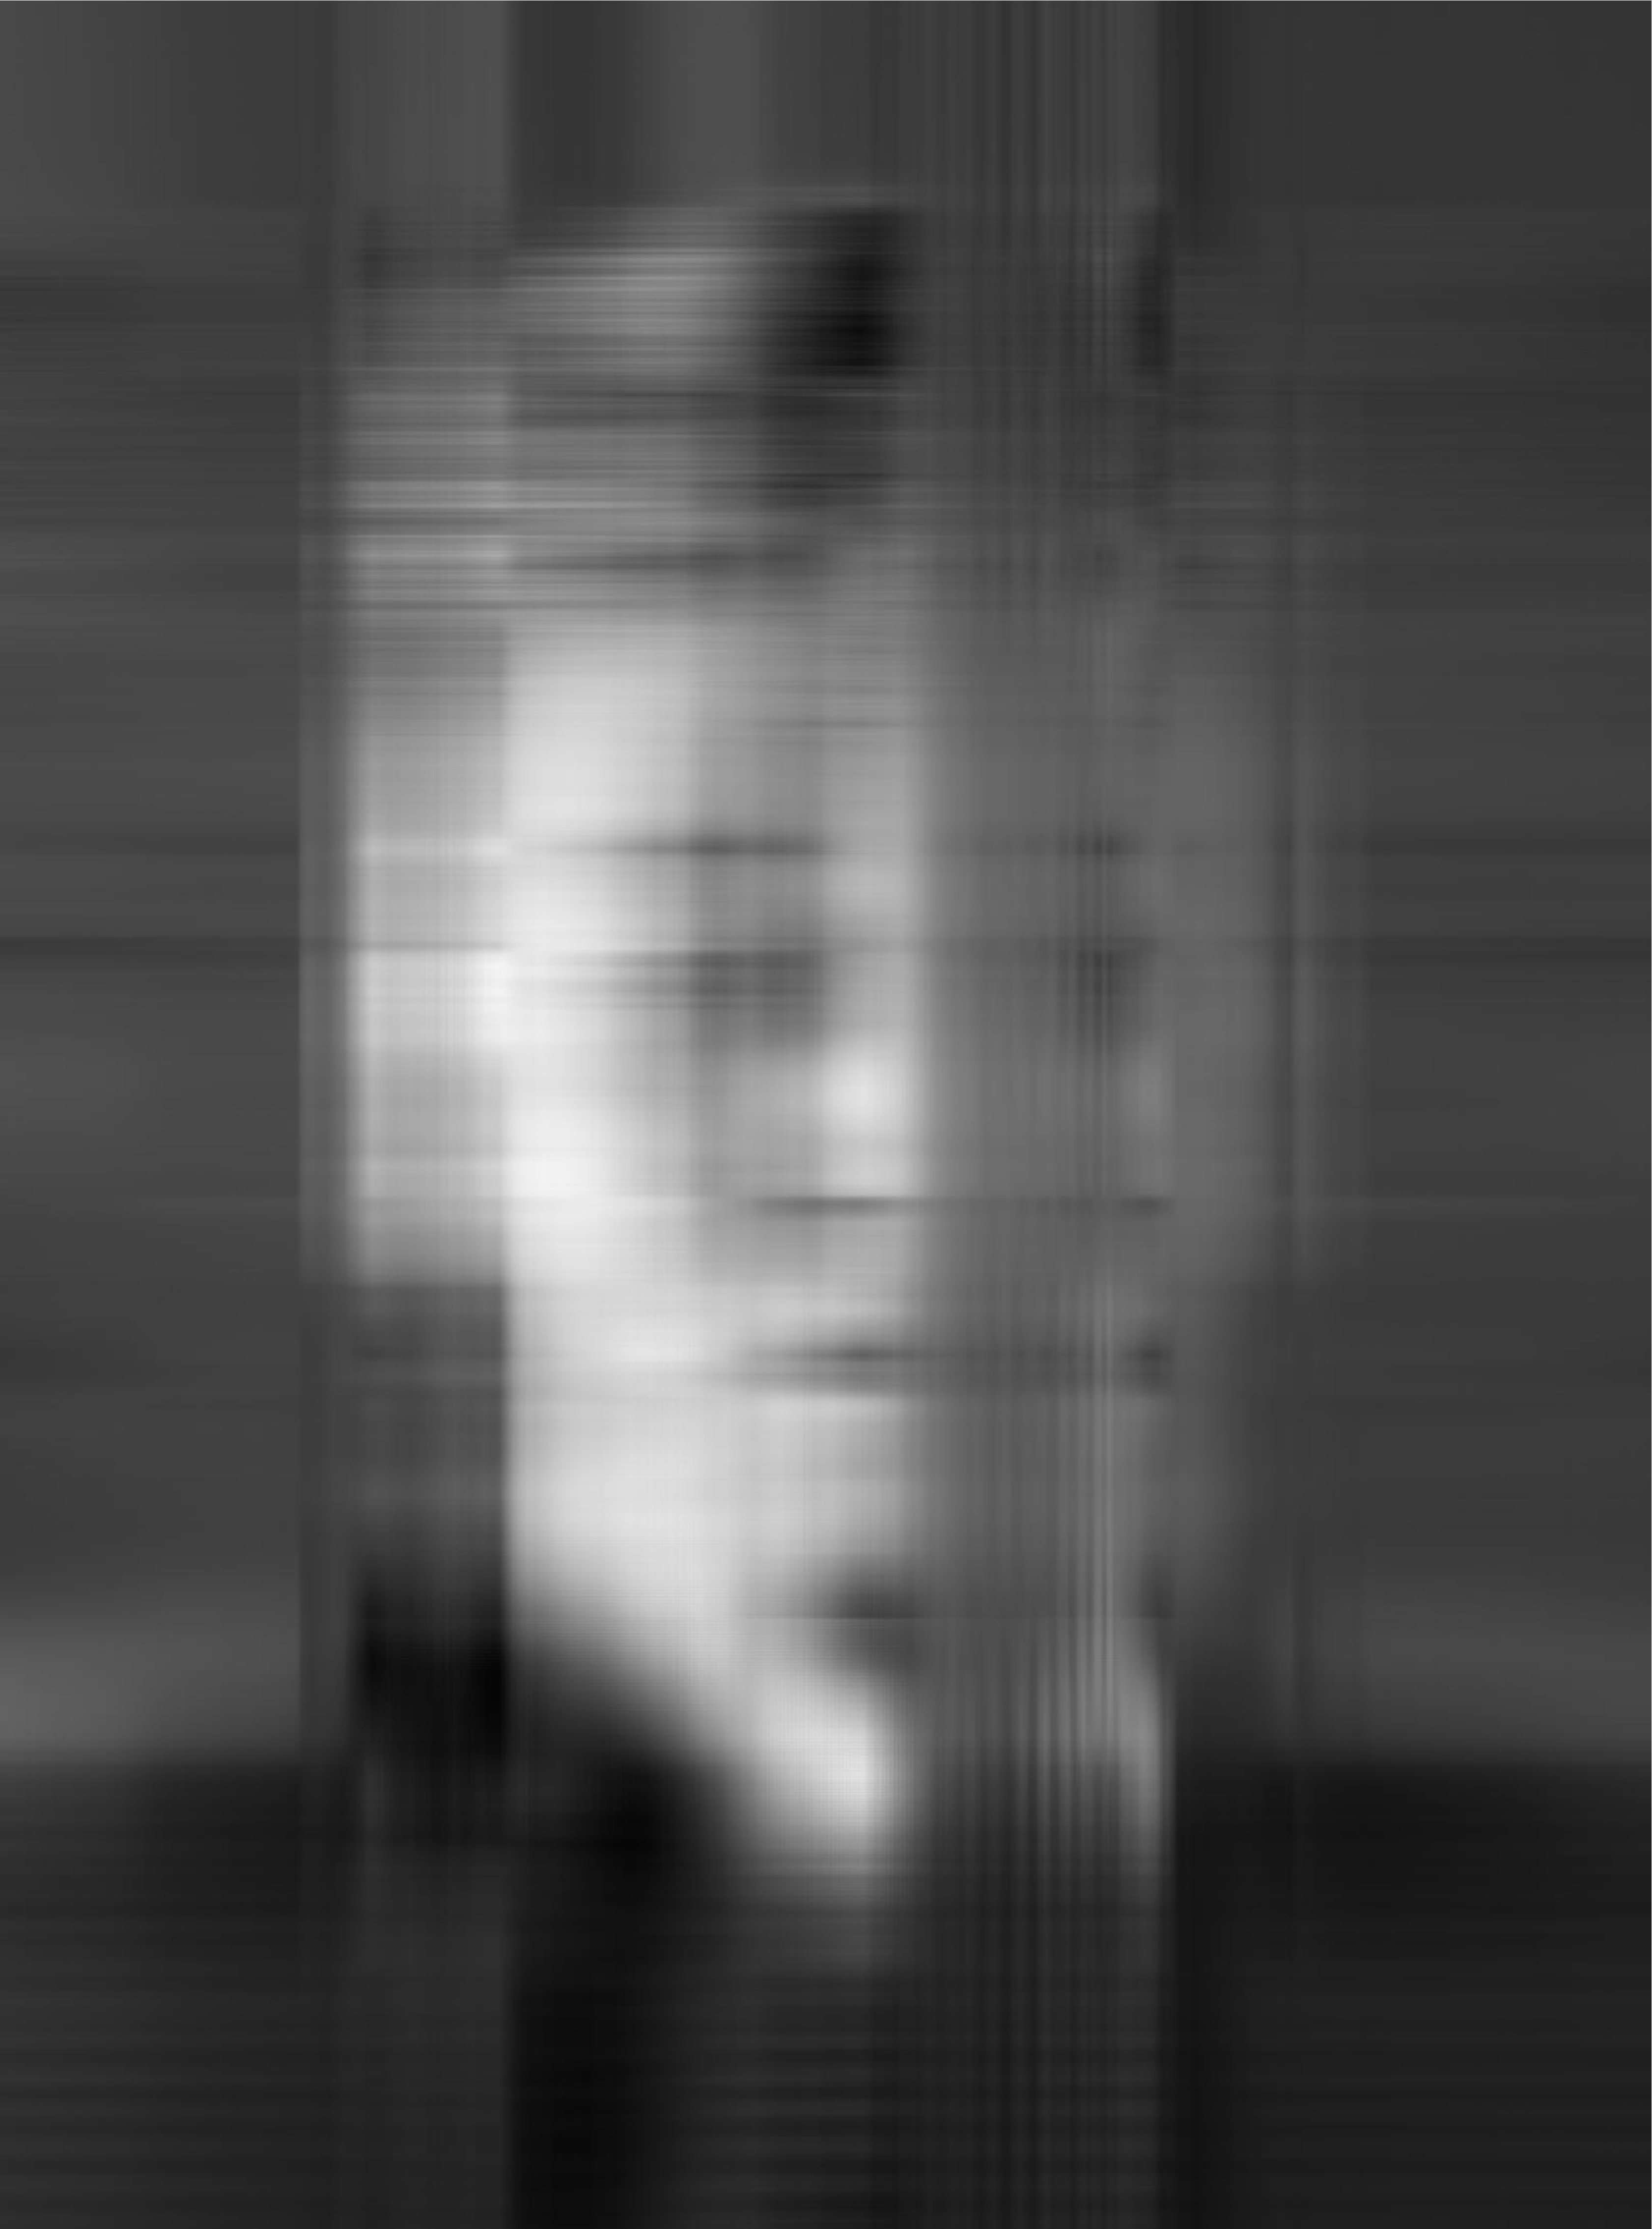
\includegraphics{image/gray_picture_r4.pdf}} \\
      $r=5$ & $r=10$ & $r=20$ & $r=50$ \\
      \resizebox{0.15\textwidth}{!}{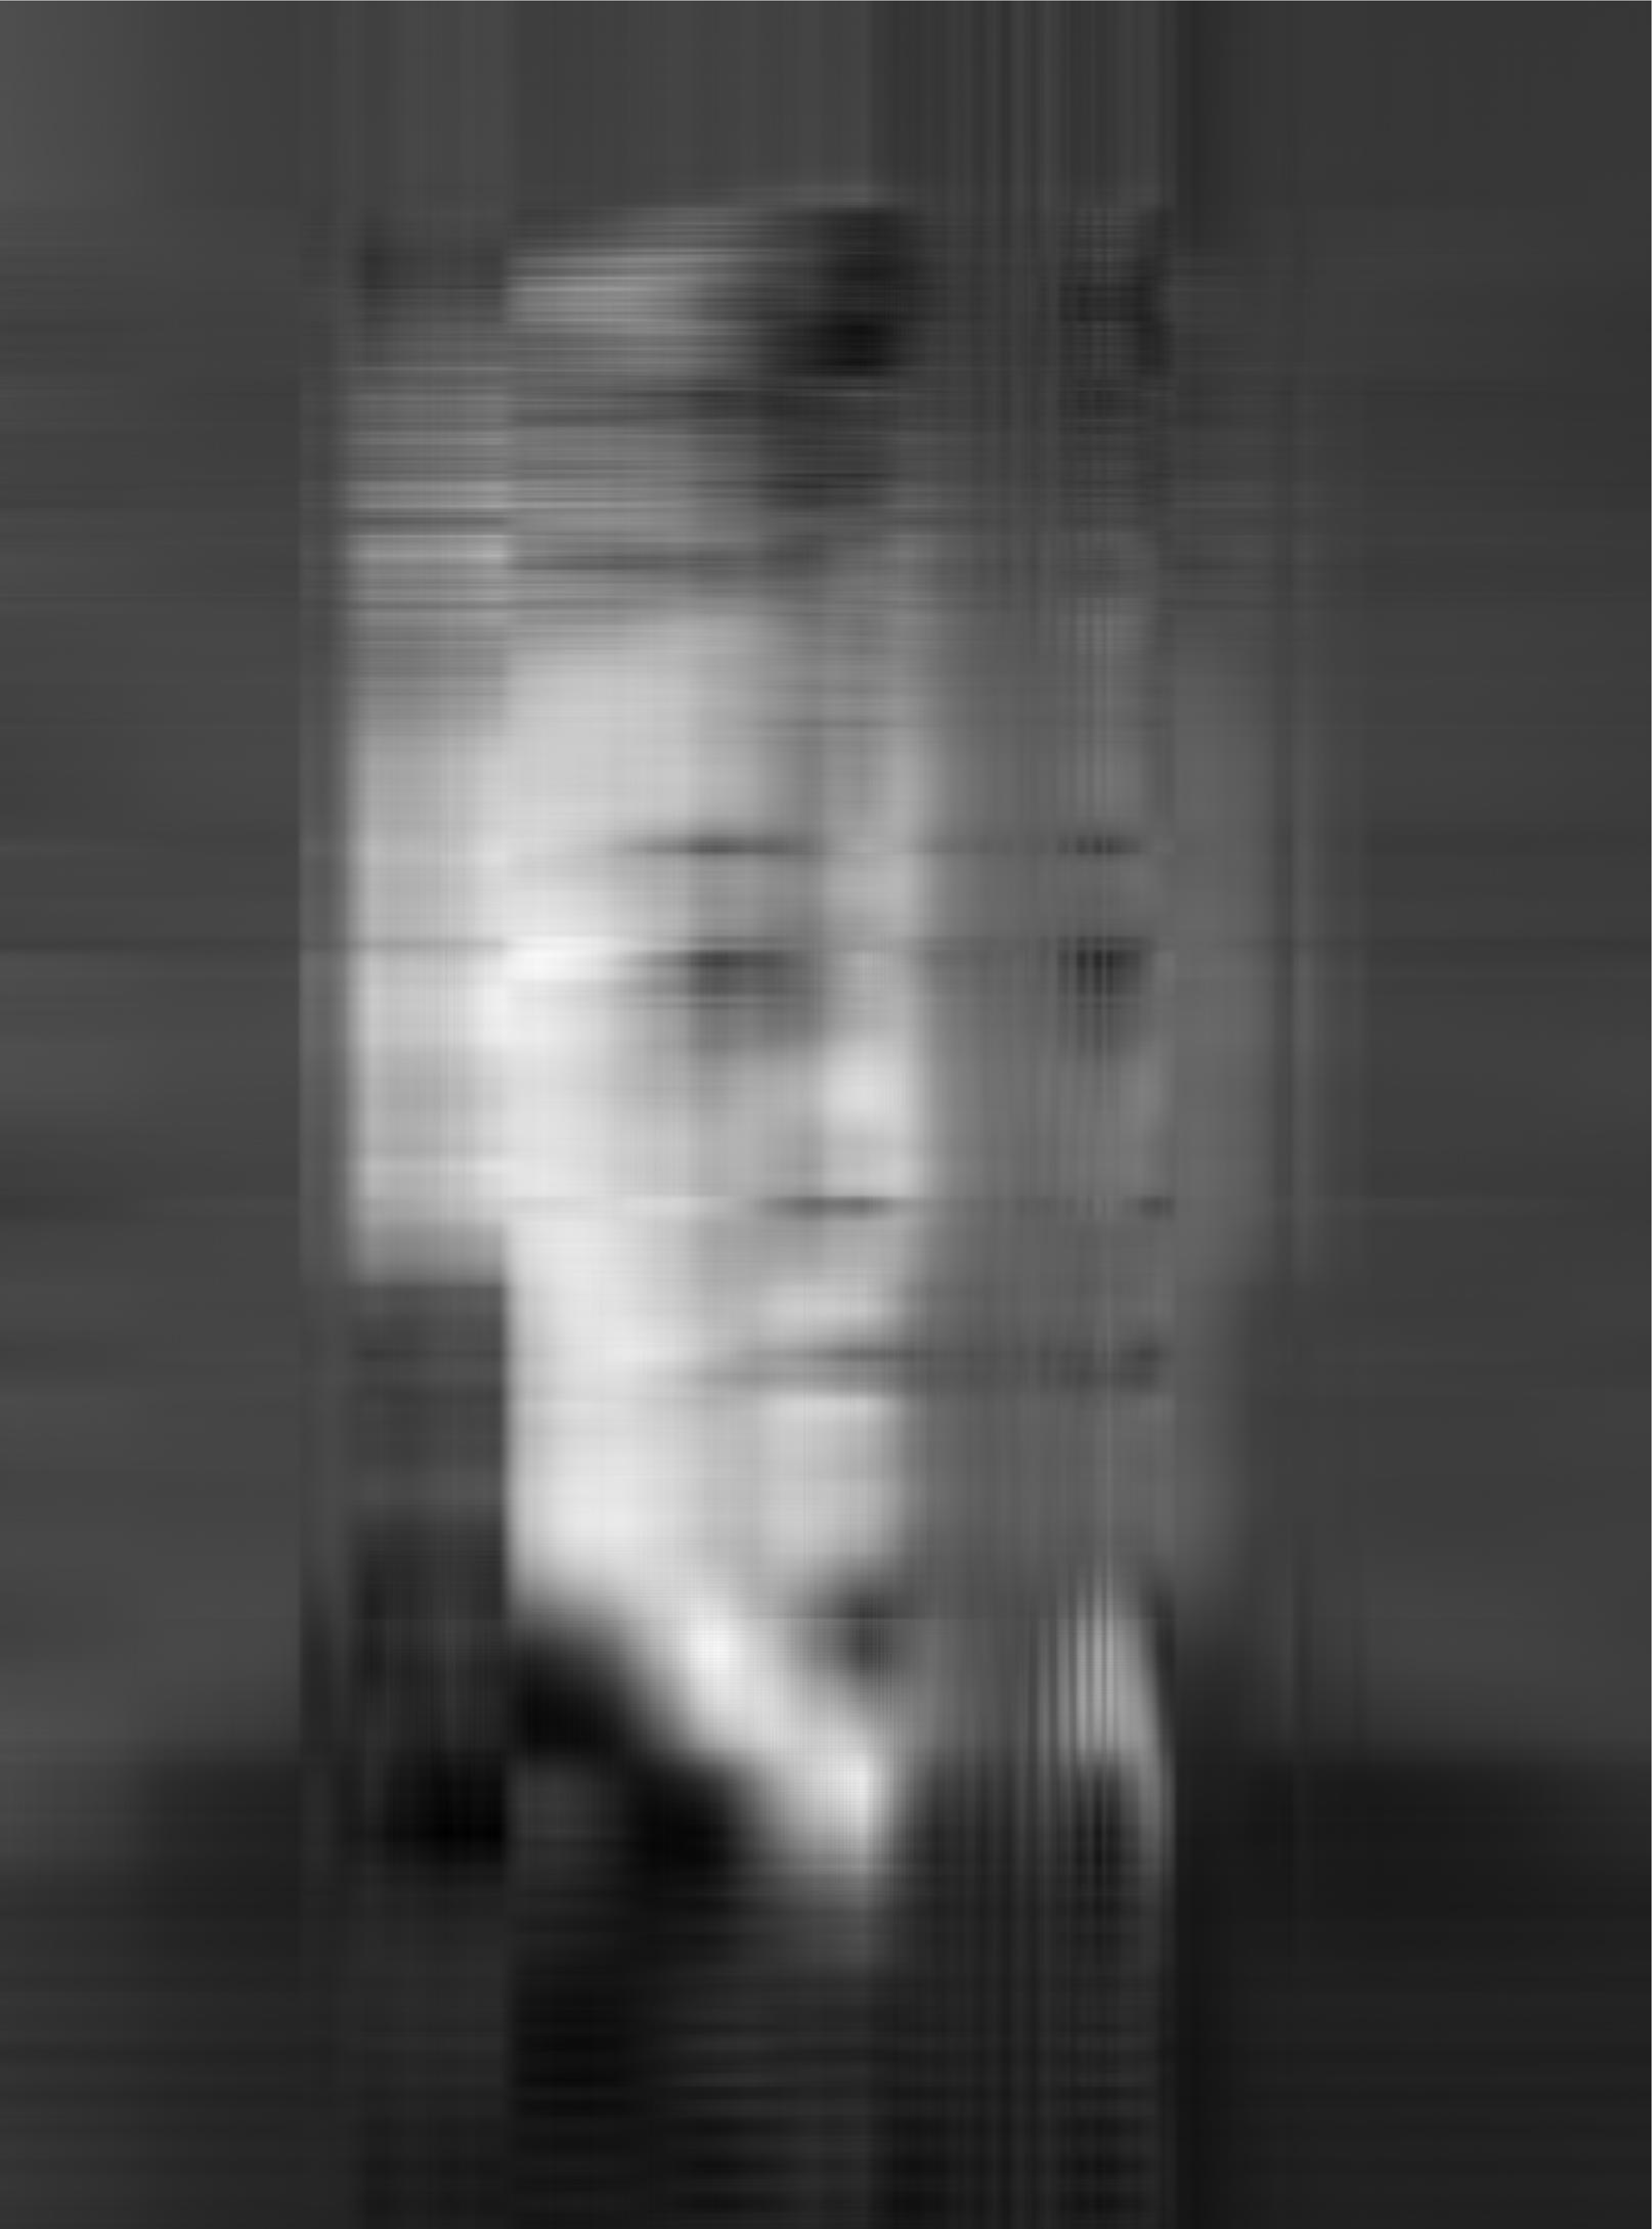
\includegraphics{image/gray_picture_r5.pdf}} &
      \resizebox{0.15\textwidth}{!}{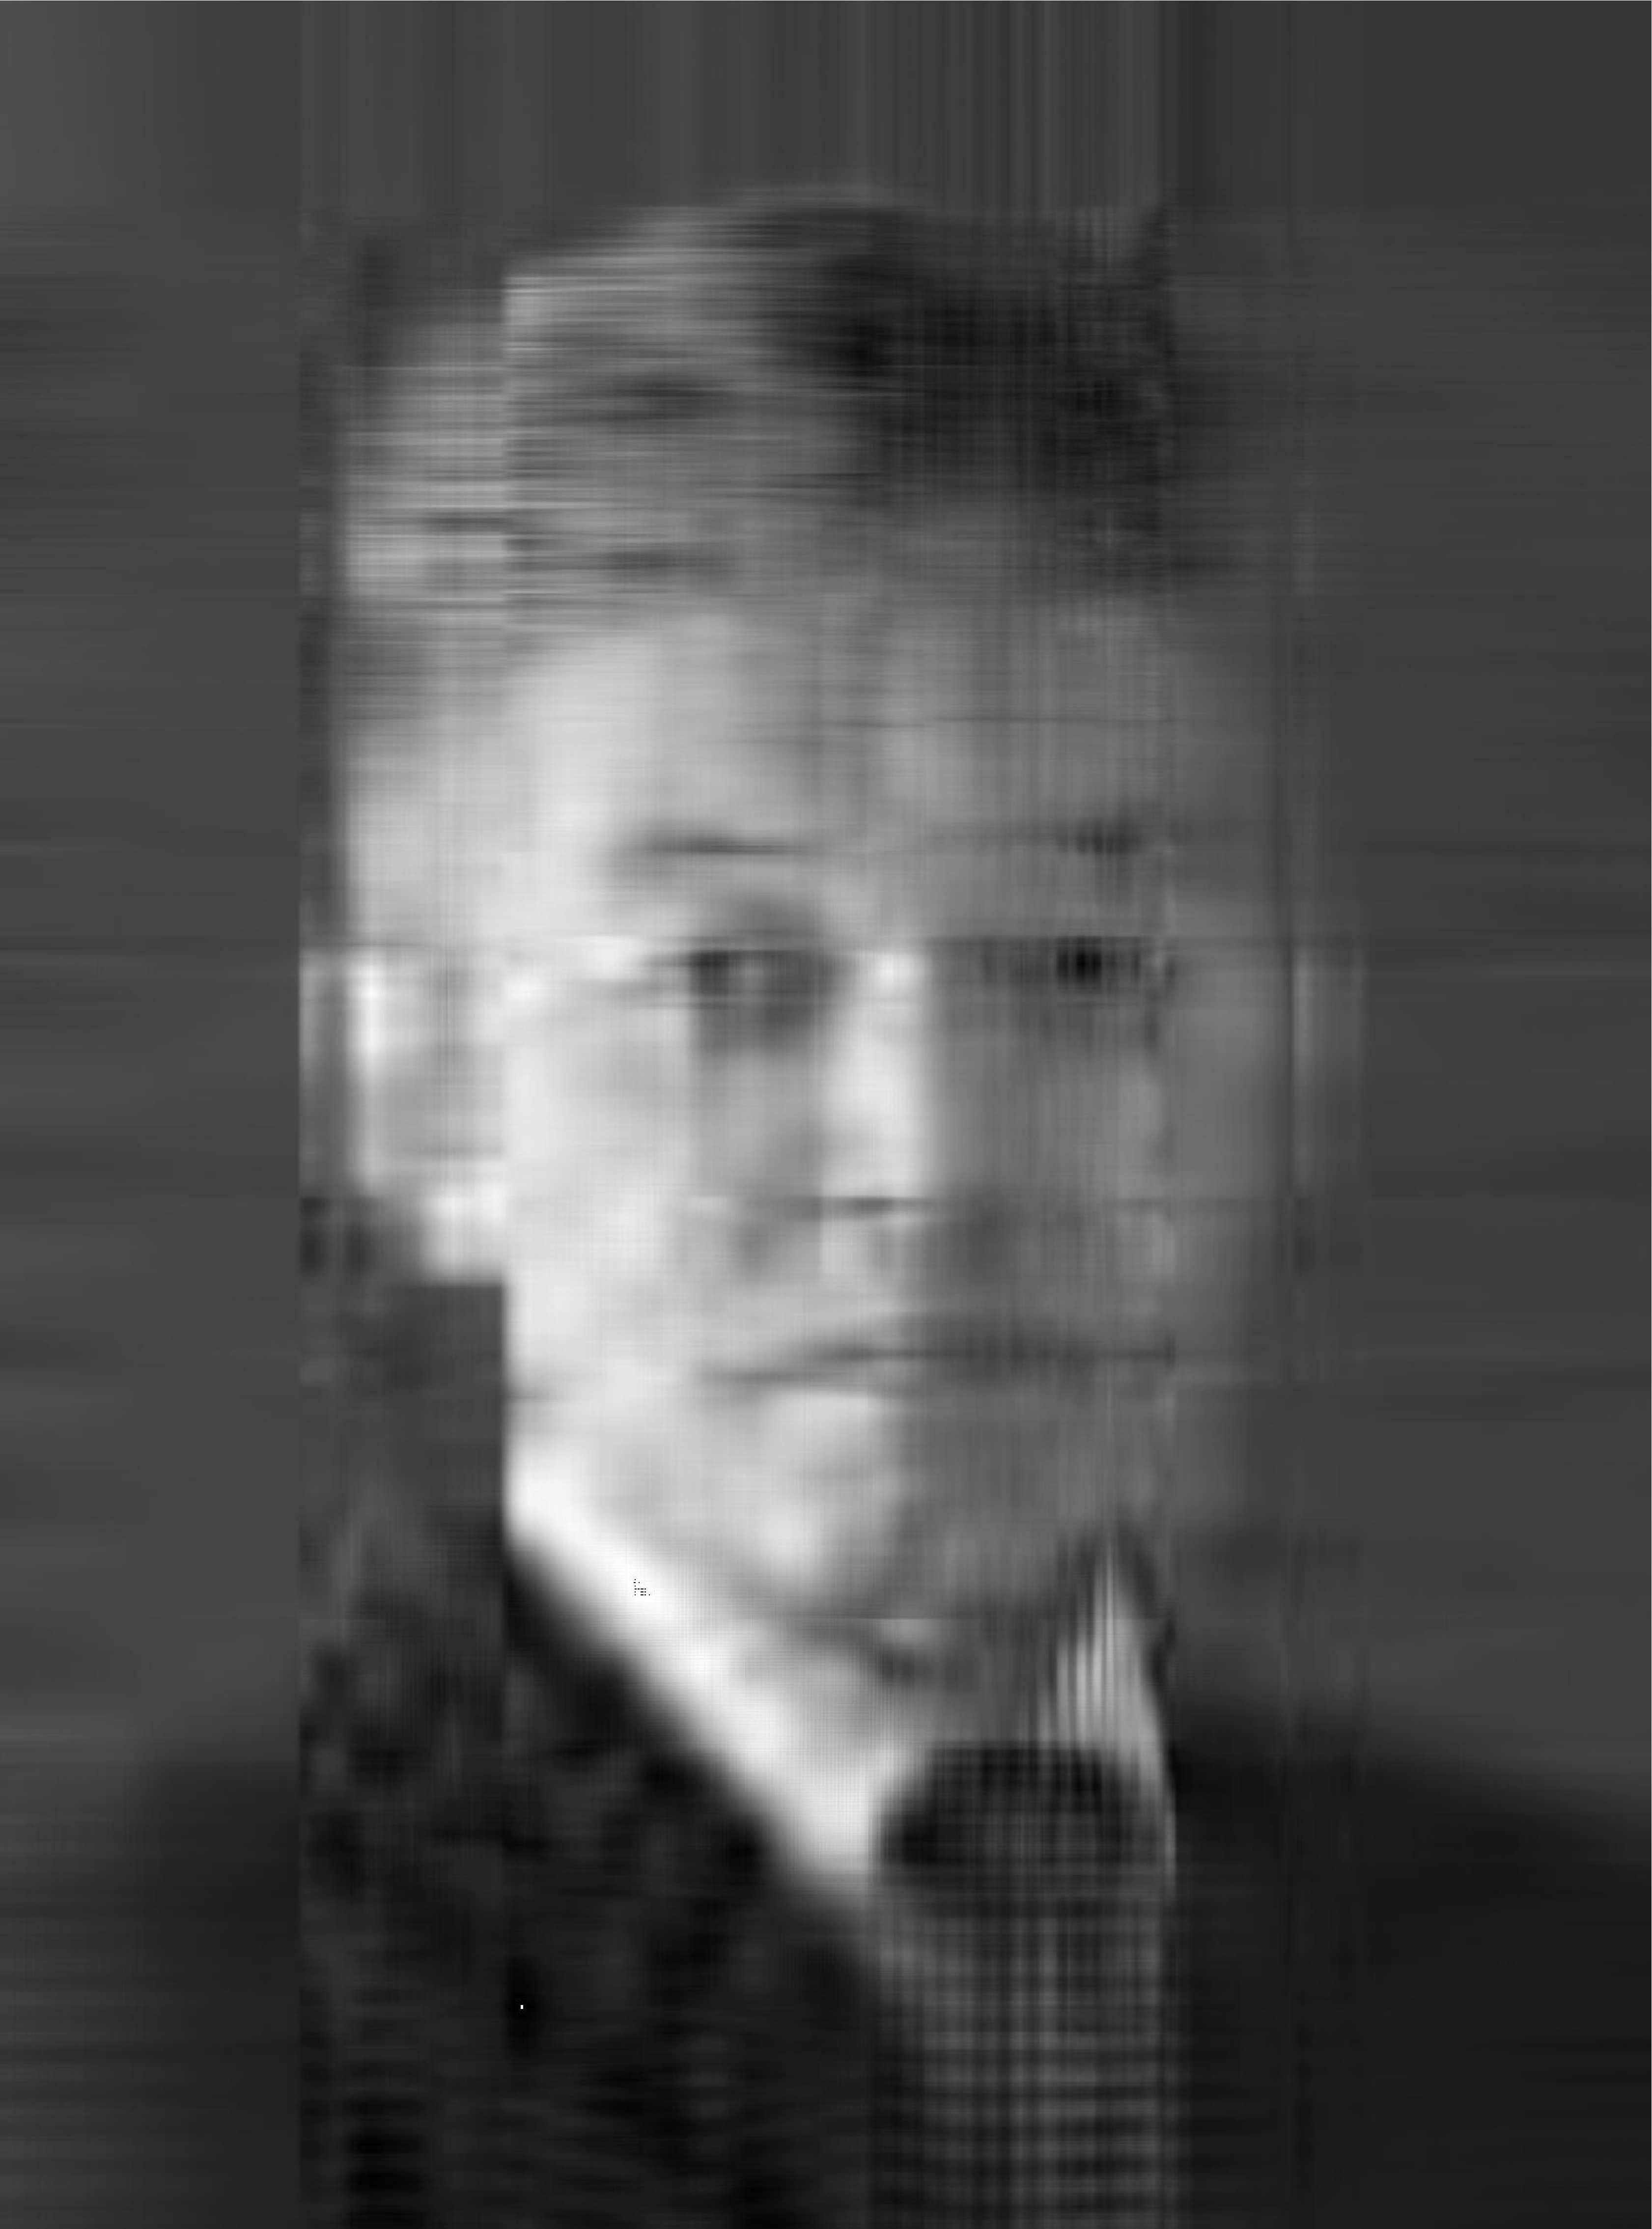
\includegraphics{image/gray_picture_r10.pdf}} &
      \resizebox{0.15\textwidth}{!}{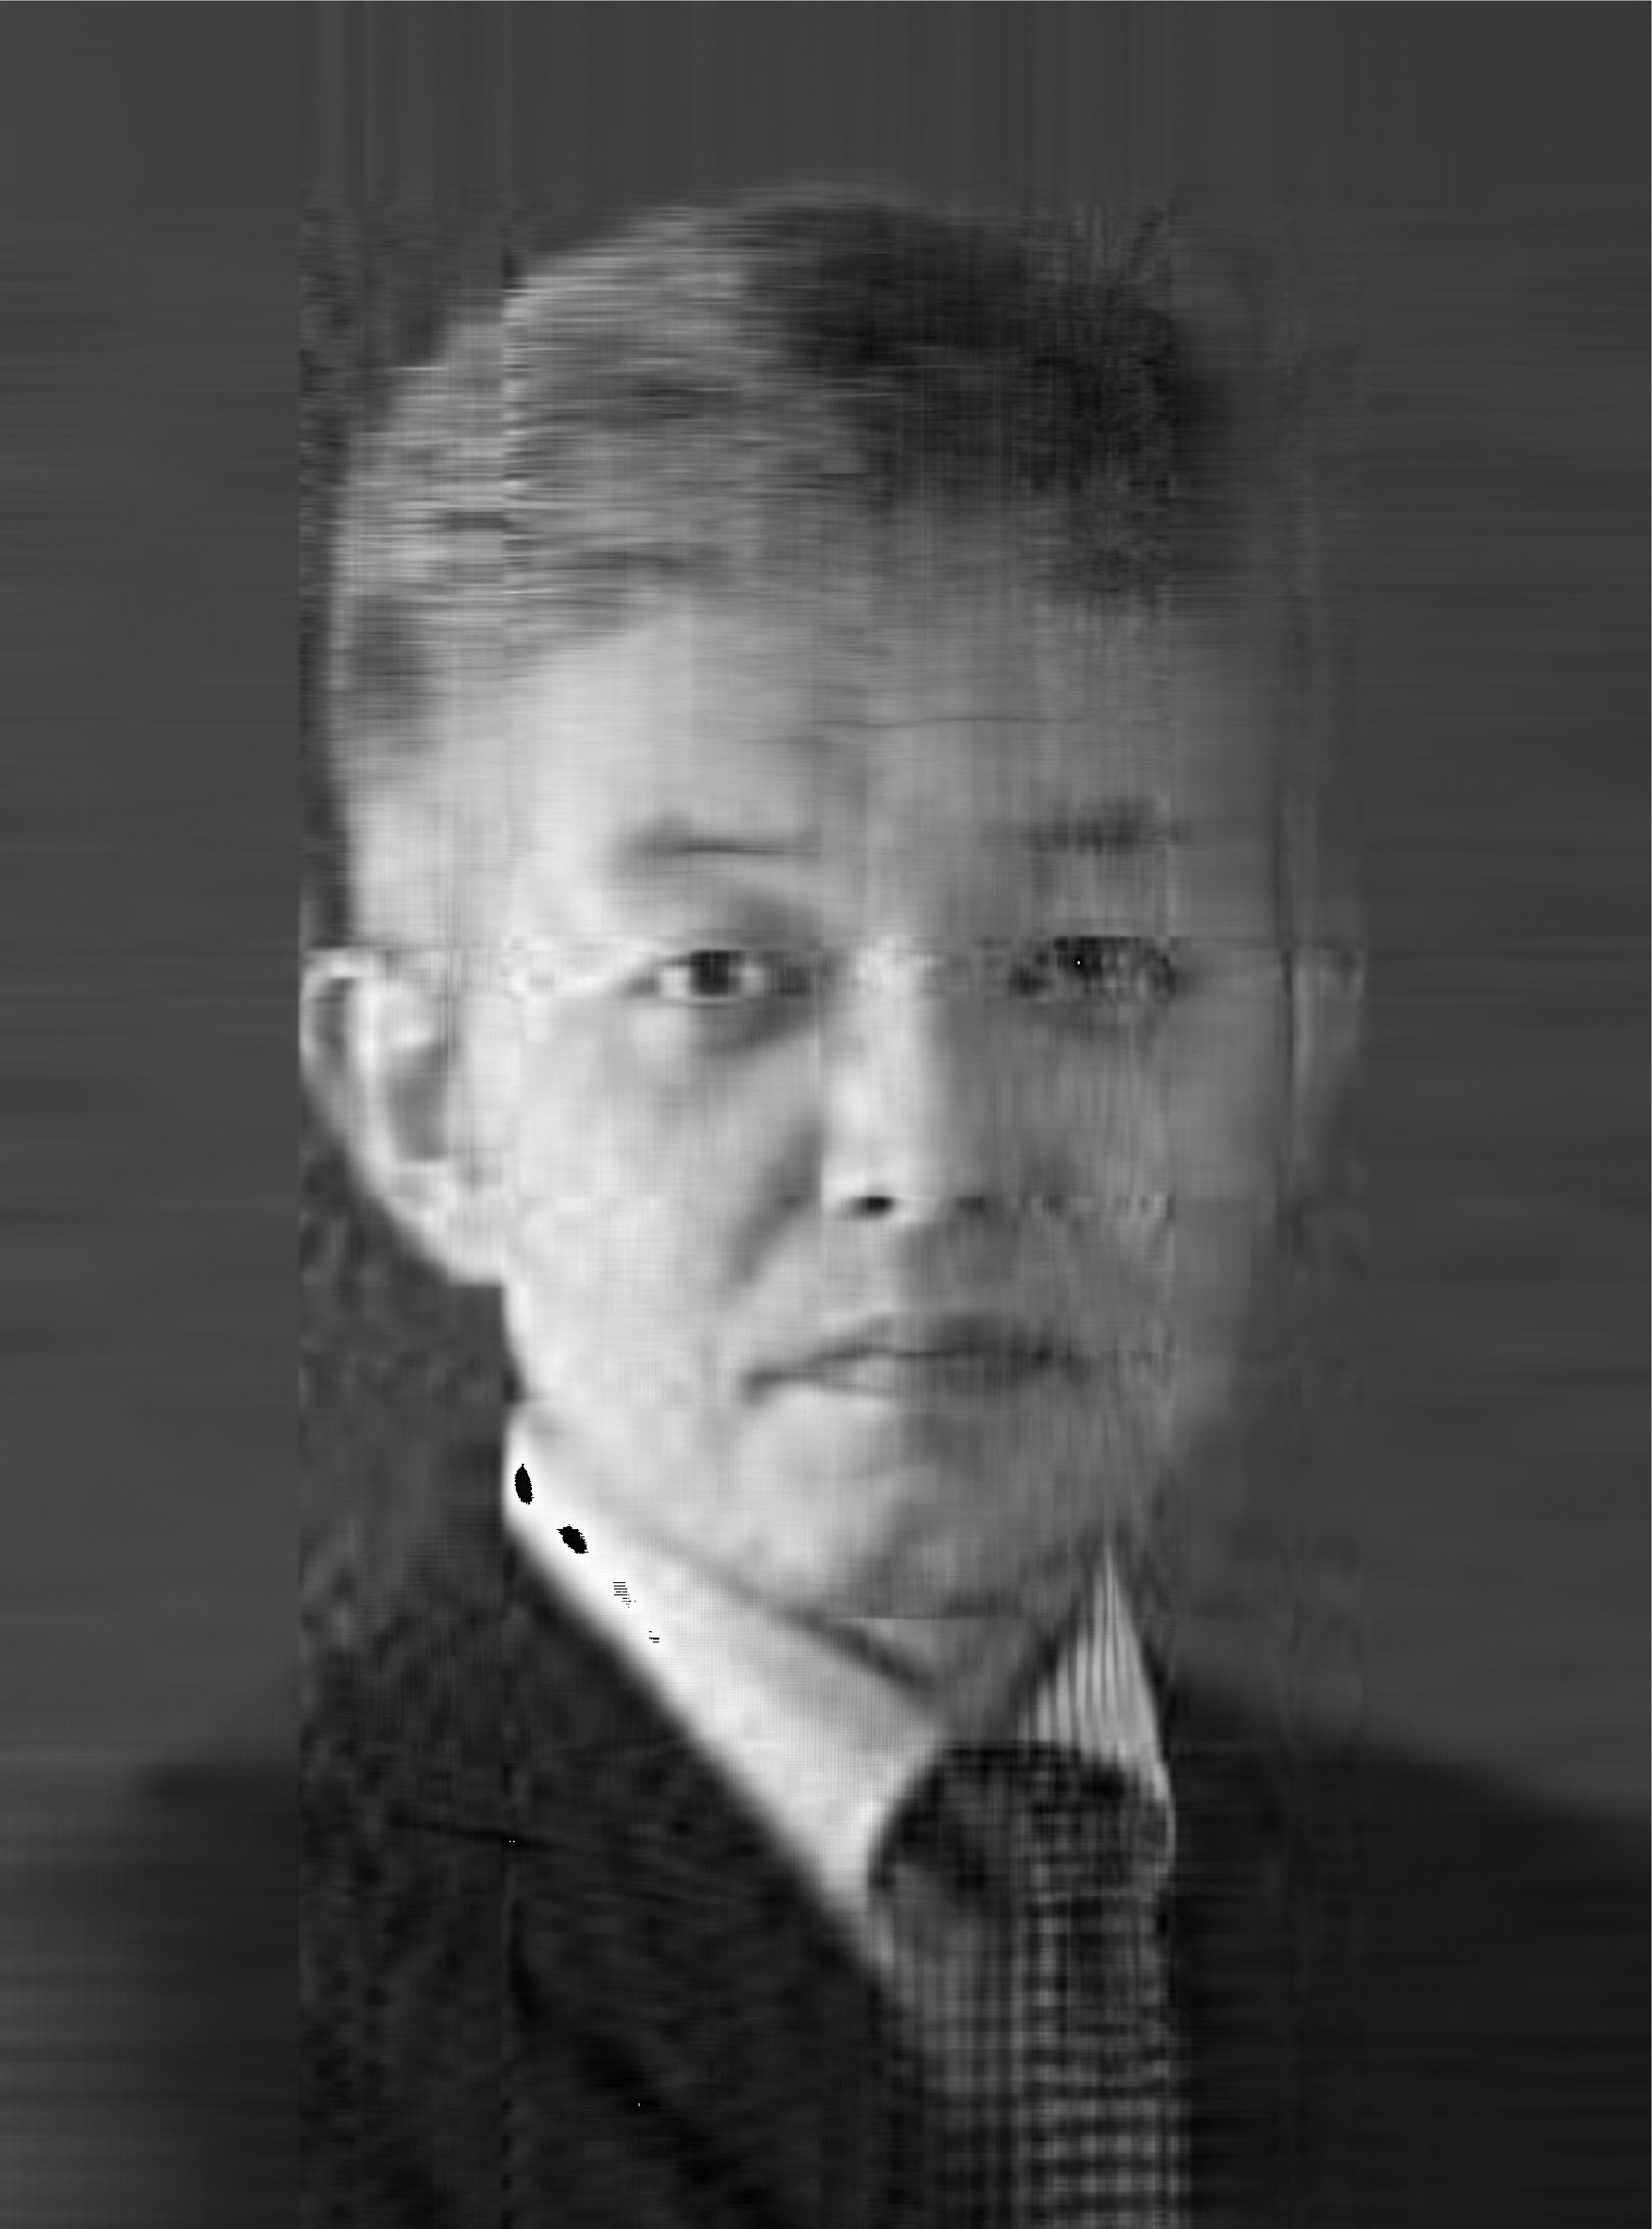
\includegraphics{image/gray_picture_r20.pdf}} &
      \resizebox{0.15\textwidth}{!}{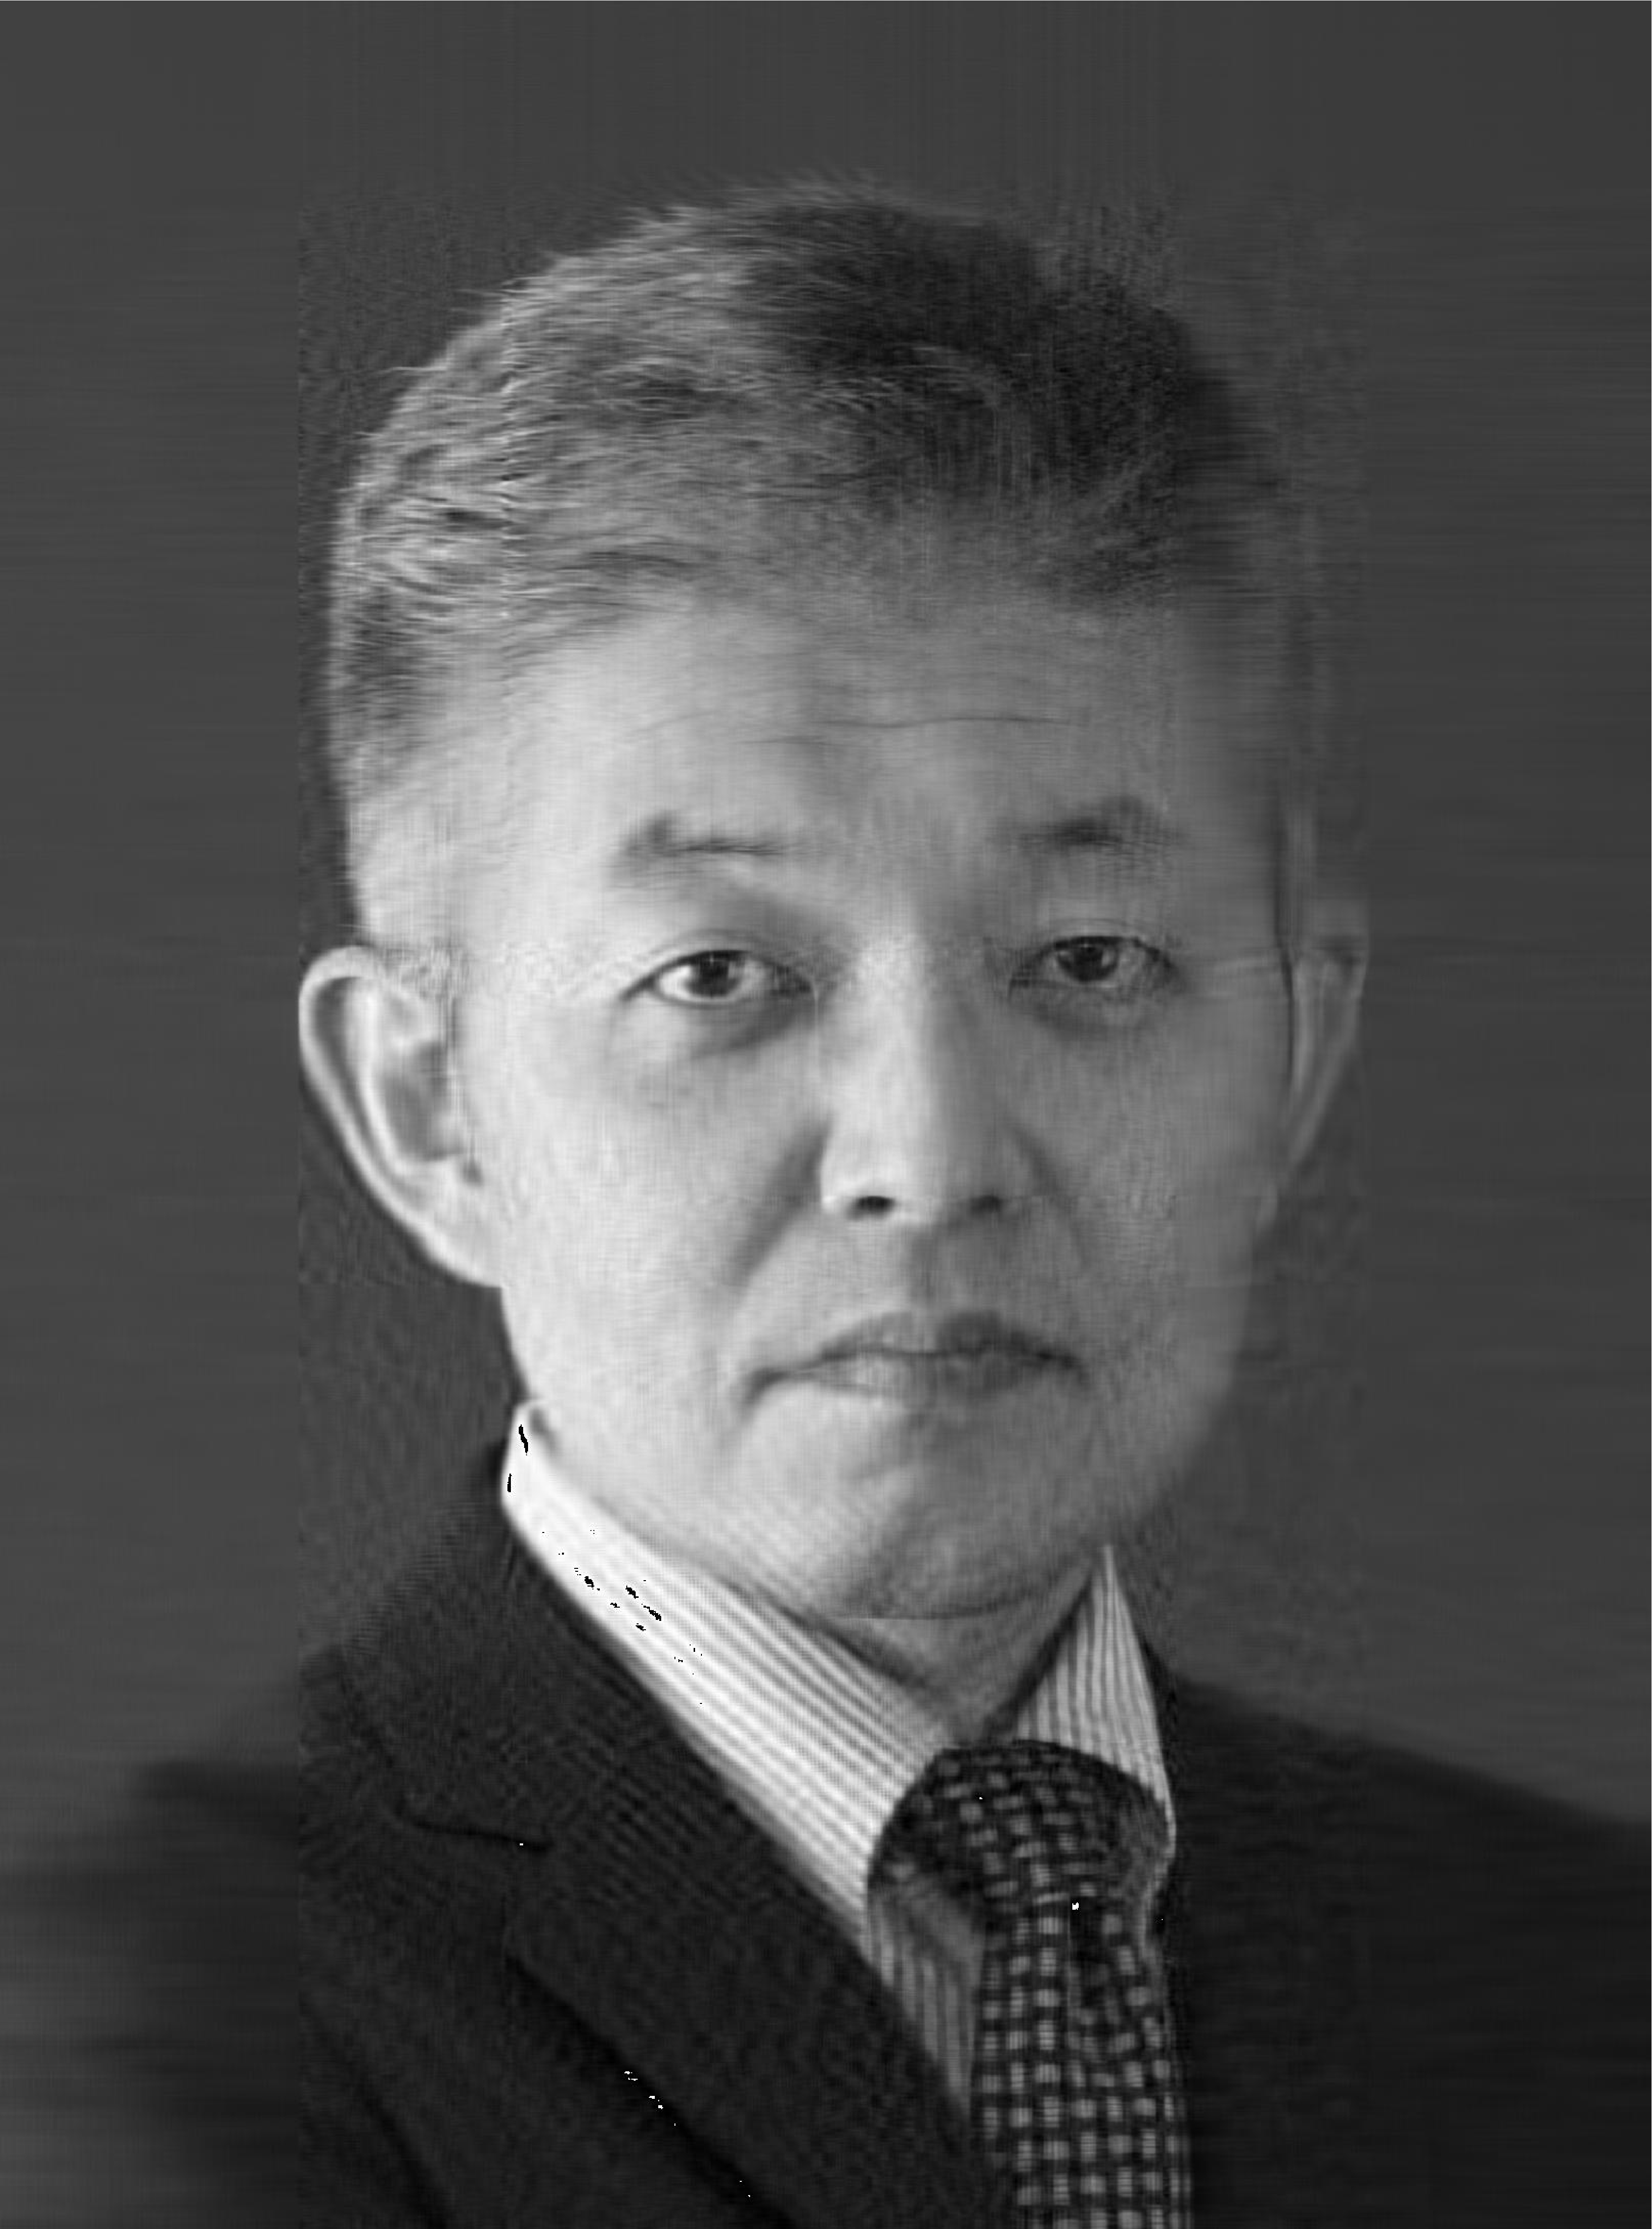
\includegraphics{image/gray_picture_r50.pdf}} \\
    \end{tabular}
  \end{itemize}
\end{frame}


\section{最小二乗法による回帰分析}

\begin{frame}[t,fragile]{最小二乗法によるフィッティング}
  \begin{itemize}
    %\setlength{\itemsep}{1em}
  \item 説明変数(例: 電圧): $x_1,x_2,x_3,\cdots,x_n$
  \item 観測値(例: 電流): $y_1,y_2,y_3,\cdots,y_n$
  \item 単回帰モデル: $y=a+bx+\epsilon$ \ \ ($\epsilon$: ノイズ)
  \item 未知母数: $a,b$
  \item 最小二乗法:
    残差$\displaystyle R(a,b) = \sum_i^n (y_i - (a+bx_i))^2$を最小化
    \[
    \begin{split}
      \frac{\partial R}{\partial a} &= - 2 \sum_i^n (y_i - (a+bx_i)) = 0 \\
      \frac{\partial R}{\partial b} &= - 2 \sum_i^n (y_i - (a+bx_i))x_i = 0
    \end{split}
    \]
  \end{itemize}
\end{frame}

\begin{frame}[t,fragile]{回帰分析の一般化}
  \begin{itemize}
    %\setlength{\itemsep}{1em}
  \item 基底関数: $\phi_j(x)$ \ \ ($j=1 \cdots m$)
  \item モデル: $\displaystyle y(x) = \sum_j^m \phi_j(x) w_j + \epsilon$
  \item 残差: $\displaystyle R({\bf w}) = \sum_i^n \Big[y_i - \sum_j^m \phi_j(x_i) w_j\Big]^2$
    \[
    \frac{\partial R}{\partial w_k} = -2 \sum_i^n \Big[ y_i - \sum_j^m \phi_j(x_i) w_j\Big] \phi_k(x_i) = 0 \qquad (k = 1\cdots m)
    \]
  \item 計画行列(design matrix) $\Phi_{ij} = \phi_j(x_i)$を導入すると
    \[
    R({\bf w}) = | {\bf y} - \Phi {\bf w} |^2
    \]
  \item 最小二乗解: $\Phi^{\rm t} \Phi {\bf w} = \Phi^{\rm t} {\bf y} \ \ \Rightarrow \ \
{\bf w} = (\Phi^{\rm t} \Phi)^{-1}\Phi^{\rm t} {\bf y}$
  \end{itemize}
\end{frame}

\begin{frame}[t,fragile]{リッジ回帰(Ridge Regression)}
  \begin{itemize}
    %\setlength{\itemsep}{1em}
  \item 基底関数の数(例: 多項式の次数)を増やしすぎると過学習 (over-fitting)」が生じる
  \item 正則化最小二乗法 ($\lambda$は非負の定数)
    \begin{align*}
    R({\bf w}) &= \sum_i^n \Big[y_i - \sum_j^m \phi_j(x_i) w_j\Big]^2 + {\color{red} \lambda} \sum_j^m w_j^2 \\
    &= | {\bf y} - \Phi {\bf w} |^2 + \lambda {\bf w}^{\rm t} {\bf w}
    \end{align*}
  \item 最小二乗解
    \[
    (\Phi^{\rm t} \Phi + \lambda \, {\rm I}) {\bf w} = \Phi^{\rm t} {\bf y} \ \ \Rightarrow \ \ 
      {\bf w} = (\Phi^{\rm t} \Phi + \lambda \, {\rm I})^{-1}\Phi^{\rm t} {\bf y}
      \]
  \end{itemize}
\end{frame}

\section{カーネル法}

\begin{frame}[t,fragile]{カーネルトリック}
  \begin{itemize}
    %\setlength{\itemsep}{1em}
  \item 方程式を変形 ${\bf w} = \frac{1}{\lambda} \Phi^{\rm t} ({\bf y} -\Phi {\bf w})$
  \item $\alpha = \frac{1}{\lambda}({\bf y} -\Phi {\bf w})$と定義すると${\bf w} =\Phi^{\rm t} \alpha$
    \item $w$は$\begin{pmatrix} \phi_1(x_1) \\ \vdots \\ \phi_M(x_1) \end{pmatrix} \cdots 
      \begin{pmatrix} \phi_1(x_N) \\ \vdots \\ \phi_M(x_N) \end{pmatrix}$の線形結合
    \item $M$次元中の$N$次元部分空間にある ($M$: 基底関数の数、$N$: サンプル数)
    \item 基底関数を増やしても自由度は増えない
    \item $w$を求める代わりに、直接$\alpha$を求めても良い (リプリゼンター定理)
  \end{itemize}
\end{frame}

\begin{frame}[t,fragile]{カーネルによる線形回帰}
  \begin{itemize}
    %\setlength{\itemsep}{1em}
  \item 残差$R$を$\alpha$をつかって表現
    \[
    R(\alpha) = | y - \Phi \Phi^{\rm t} \alpha |^2 + \lambda \alpha^{\rm t} \Phi \Phi^{\rm t} \alpha
    \]
  \item グラム行列(Gram matrix) $K \equiv \Phi \Phi^{\rm t}$を導入すると
    \[
    R(\alpha) = | y - K \alpha |^2 + \lambda \alpha^{\rm t} K \alpha
    \]
  \item グラム行列($N \times N$対称行列)の成分
    \[
    K_{ik} = \sum_j \Phi_{ij} \Phi_{kj} = \sum_j \phi_j(x_i) \phi_j(x_k) \equiv {\color{red} k(x_i,x_k)}
    \]
  \item $M$個の基底関数の組を考えるかわりに1つのカーネル関数$k(x,x')$を導入すればよい(カーネル法)
  \end{itemize}
\end{frame}

\begin{frame}[t,fragile]{カーネルによる線形回帰}
  \begin{itemize}
    %\setlength{\itemsep}{1em}
  \item 残差$R$の最小化
    \[
    \alpha = (K + \lambda \, {\rm I})^{-1} {\bf y}
    \]
  \item 点$x$における$y$の推定値
    \begin{align*}
    y &= \sum_j \phi_j(x) w_j = \sum_{i,j} \phi_j(x) \phi_j(x_i) \alpha_i = \sum_i k(x_i,x) \alpha_i \\ &= k^{\rm t}(x) \alpha = k^{\rm t}(x) (K + \lambda \, {\rm I})^{-1} {\bf y}
k(x) = \begin{pmatrix} k(x_1,x) \\ k(x_2,x) \\ \vdots \\ k(x_N,x) \end{pmatrix}
    \end{align*}
  \item 例: ガウシアンカーネル $k(x,x') = \exp(-\beta|x-x'|^2)$
  \end{itemize}
\end{frame}

\section{ベイズ統計の基礎}

\begin{frame}[t,fragile]{条件付き確率}
  \begin{itemize}
    \setlength{\itemsep}{1em}
  \item 子供が二人いる家族において「二人の子供のうち少くとも一人が女の子である場合」二人とも女の子である確率は?
  \item 日本人の{\color{red} 1/10000}がウイルスAに感染しているとする。このウイルスに感染していると、{\color{red} 999/1000}の確率で検査で陽性となる。一方、感染していなくても、{\color{red} 1/100}の確率で陽性となってしまう(偽陽性)。検査結果が陽性の場合、感染している可能性は?
    \begin{itemize}
    \item 事象A:ウイルスに感染
    \item 事象B:検査で陽性
    \end{itemize}
  \end{itemize}
\end{frame}

\begin{frame}[t,fragile]{ベイズの定理}
  \begin{itemize}
    %\setlength{\itemsep}{1em}
  \item 確率に対する公式
    \begin{align*}
      P(A \cap B) &= P(B|A) P(A) = P(A|B) P(B) \\ P(B) &= P(B|A) P(A) + P(B|\bar{A}) P(\bar{A})
    \end{align*}
  \item ベイズの定理 (確率の反転)
    \[
    P(A|B) = \frac{P(B|A)P(A)}{P(B)} = \frac{P(B|A)P(A)}{P(B|A) P(A) + P(B|\bar{A}) P(\bar{A})}
    \]
  \item 検査が陽性でも、実際に感染している可能性(確率)は
    \[
    \frac{\frac{999}{1000} \cdot \frac{1}{10000}}{\frac{999}{1000} \cdot \frac{1}{10000} + \frac{1}{100} \cdot \frac{9999}{10000}} \approx {\color{red} 0.009}
    \]
    \begin{itemize}
    \item 予想よりずっと小さい?
    \item 「検査が陽性」という事実により、感染している確率が 0.01\%から 0.9\%に増加 $\Rightarrow$ ベイズ統計・機械学習の基礎公式
    \end{itemize}
  \end{itemize}
\end{frame}

\begin{frame}[t,fragile]{ベイズ統計学(Bayesian Statistics)}
  \begin{itemize}
    %\setlength{\itemsep}{1em}
  \item 条件つき確率におけるベイズの定理
    \[
    p(\theta|y) \sim p(y|\theta) p(\theta)
    \]
  \item この(あたりまえの)関係式をベイズ統計では以下のように解釈する
    \begin{itemize}
    \item $\theta$未知母数(パラメータ) : 物理量の平均、分散、比例係数、etc
    (確定した値ではなくある分布に従って変動する量として考える)
    \item $y$ 観測値 : すでに「与えられた」確定したものと考える
    \item $p(\theta)$ 事前確率 (prior probability) : 母数に関する何らかの事前情報
    \item $p(y|\theta)$ 尤度 (likelihood) : $y$は与えられている$\theta$の関数と解釈。$l(\theta|y)$ と書く
    \item $p(\theta|y)$ 事後確率 (posterior probability) : 観測で情報が増えた後の$\theta$の確率分布
    \end{itemize}
  \end{itemize}
\end{frame}

\begin{frame}[t,fragile]{頻度主義的アプローチとベイズ的アプローチ}
  \begin{itemize}
    %\setlength{\itemsep}{1em}
  \item コインを一回投げて表が出る確率 $q$
  \item 連続して三回連続して表が出る($y$)確率 $p(y|q) = q^3 = l(q|y)$  ($q$ の尤度関数)
  \item 頻度主義的アプローチ(最尤推定)
    \begin{itemize}
    \item $q$ の推定値 $q=1$ \ \ $\Rightarrow$ \ \ 未来永劫表が出続ける!
    \item 観測データ数$\sim$母数の数の時 \ \ $\Rightarrow$ \ \ 過学習(over-fitting)
    \end{itemize}
  \item ベイズ的アプローチ
    \begin{itemize}
    \item $q$の事前分布として $p(q) = 1$  \ \ $\Rightarrow$ \ \ %事後分布
      $p(q|y) \sim l(q|y) p(q) = q^3$
    \end{itemize}
  \item ベイズ的アプローチでは過学習の問題が生じない
  \item 有効パラメータ数が自動的にデータ集合のサイズに適合
  \end{itemize}
\end{frame}

\begin{frame}[t,fragile]{回帰分析への応用}
  \begin{itemize}
    %\setlength{\itemsep}{1em}
  \item 単回帰モデル: $y=a+bx+\epsilon$ \ \ ($\epsilon$: ノイズ)
  \item 尤度関数 (likelihood function) :
    \[
    l(a, b | \{x_i\}, \{y_i\}) = p(\{y_i\} | \{x_i\}, a, b) \sim \prod_i \exp \Big[ -\frac{(y_i - (a+bx_i))^2}{2\sigma^2}\Big]
    \]
  \item 事前分布を導入
    \begin{itemize}
    \item 例えば $a$, $b$ について ${\cal N}(0,1000)$
    \end{itemize}
  \item 事後分布:
    \[
    p(a,b | \{x_i\}, \{y_i\}) \sim l(a, b | \{x_i\}, \{y_i\}) p(a) p(b)
    \]
    \begin{itemize}
      \item $a$, $b$ の事後周辺分布から期待値とその確からしさを推定
      \item 最大事後確率(MAP)推定
    \end{itemize}
  \end{itemize}
\end{frame}

\begin{frame}[t,fragile]{最小二乗法・カーネル法・ベイズ推定}
  \begin{itemize}
    \setlength{\itemsep}{1em}
  \item 非線形最小二乗法
    \begin{itemize}
    \item 非線形の最小化問題
    \end{itemize}
  \item カーネル法
    \begin{itemize}
    \item 実質的に無限次元の問題を解くことができる
    \item データサイズが大きくなるとその3乗に比例して計算量が増大
    \end{itemize}
  \item ベイズ推定
    \begin{itemize}
    \item 事後確率をコンパクトな形で求めることは難しい
    \item モンテカルロ法の利用
    \end{itemize}    
  \end{itemize}
\end{frame}


\begin{frame}[t]{本日の課題}
  \begin{itemize}
    %\setlength{\itemsep}{1em}
  \item 「\href{https://utphys-comp.github.io}{計算機実験のための環境整備}」({\small \href{https://utphys-comp.github.io}{https://utphys-comp.github.io}})が完了していない人は至急連絡を!
  \item 実習
    \begin{itemize}
    \item 実習課題一覧\href{https://github.com/todo-group/ComputerExperiments/releases/tag/2020s-computer1}{exercise-1.pdf}の課題17〜24 (あるいはそれ以外)から適宜選び実習
    \end{itemize}
  \item 質問はSlackの「\# 5\_対角化」あるいは他の適当と思われるチャンネルで \\[2em]
  \item レポートNo.3: 提出締切2020/7/3(金) 18:00 (レポート内容・提出方法についてはITC-LMSを参照のこと)
  \item 
  \end{itemize}
\end{frame}

\end{document}
